\documentclass[11pt,a4paper]{article}

\usepackage[T1]{fontenc}
\usepackage[utf8]{inputenc}
\usepackage[spanish,es-noquoting]{babel}
\usepackage{mathptmx}\usepackage[scaled=.9]{helvet}
\usepackage{amsmath,amssymb}
\usepackage{graphicx}
\usepackage{booktabs}
\usepackage{xcolor}
\usepackage[margin=2.3cm]{geometry}
\usepackage[colorlinks=true,linkcolor=azulq,citecolor=azulq,urlcolor=azulq]{hyperref}
\usepackage{caption}
\usepackage{enumitem}
\usepackage{float}
\usepackage{longtable}
\usepackage{array}

\definecolor{azulq}{HTML}{1F3B59}
\definecolor{cuantico}{HTML}{5347C4}
\definecolor{clasico}{HTML}{A8651F}
\definecolor{fiel}{HTML}{2F7A5C}
\definecolor{alarma}{HTML}{A02C2C}

\captionsetup{font=small,labelfont={bf,color=azulq}}

\newcommand{\Cu}[1]{\textcolor{cuantico}{\textbf{#1}}}
\newcommand{\Cl}[1]{\textcolor{clasico}{\textbf{#1}}}
\newcommand{\Fi}[1]{\textcolor{fiel}{\textbf{#1}}}
\newcommand{\Al}[1]{\textcolor{alarma}{\textbf{#1}}}

% Caja de "qué contesta" al inicio de cada figura.
\newcommand{\contesta}[1]{%
  \par\medskip\noindent
  \colorbox{azulq!8}{%
    \begin{minipage}{\dimexpr\textwidth-2\fboxsep}
    \small\textbf{\textcolor{azulq}{Qué contesta:}} #1
    \end{minipage}}\par\medskip}

\newcommand{\archivo}[1]{\par\noindent\textbf{Archivo:} \texttt{#1}\par}

\title{\bfseries Guía de figuras\\[.3em]
  \large Qué contesta cada gráfica del proyecto,\\
  con un ejemplo real de cada tipo}
\author{Andrés García Rivera}
\date{\today}

\begin{document}
\maketitle

\begin{abstract}
\noindent
El proyecto produce unas cuatrocientas figuras por campaña, de catorce tipos
distintos. Este documento enseña a leer cada tipo: qué hay en cada eje, qué
pregunta contesta, qué hay que mirar primero y qué cuenta como un valor
alarmante. Todos los ejemplos son figuras reales de la campaña
\texttt{hpc\_20260907\_182345} (Saptiva), no ilustraciones hechas a mano.

\medskip\noindent
La regla que ordena todo el documento: \textbf{cada figura contesta una
pregunta}. Si no sabes qué pregunta contesta, no la metas en el paper.
\end{abstract}

\tableofcontents
\bigskip

% =====================================================================
\section{Los tres ejes}
% =====================================================================

Todo el marco se mueve en tres ejes independientes, y cada figura vive en uno
de ellos. Saber en cuál está es la mitad de leerla.

\begin{center}
\small
\begin{tabular}{@{}>{\raggedright\arraybackslash}p{3.3cm}>{\raggedright\arraybackslash}p{6.2cm}>{\raggedright\arraybackslash}p{5.6cm}@{}}
\toprule
\textbf{eje} & \textbf{qué se mueve} & \textbf{figuras} \\
\midrule
tamaño del registro
  & \texttt{nqpp} (qubits por parámetro, en los samplers) o \texttt{n\_bits}
    (bits por gen, en el genético)
  & \texttt{convergence\_*}, \texttt{cost\_*}, \texttt{ruido\_vs\_rejilla\_*} \\
\addlinespace
quantumness
  & de $0\%$ a $100\%$ de componentes cuánticos encendidos
  & \texttt{ladder\_*}, \texttt{corner\_ladder\_*}, \texttt{fitness\_*} \\
\addlinespace
ruido
  & \texttt{none} / \texttt{readout} / \texttt{full} / \texttt{FakeBrisbane}
  & \texttt{ruido\_vs\_rejilla\_*}, \texttt{ruido\_fijo\_*} \\
\bottomrule
\end{tabular}
\end{center}

\noindent
\textbf{Ojo con una trampa:} \texttt{nqpp} y \texttt{n\_bits} viven en la
\emph{misma} columna del CSV pero \textbf{no son la misma cantidad}. Para los
samplers es cuántos qubits se usan por cada parámetro de la rejilla del
posterior; para el genético es cuántos bits tiene cada gen de la codificación.
Ponerlas en un mismo eje junta dos números incomparables. Por eso las figuras
del genético llevan el sufijo \texttt{\_genetico} y su propio eje: son dos
figuras separadas, a propósito.

% =====================================================================
\clearpage
\section{Por campaña: la carpeta \texttt{hpc\_*}}
% =====================================================================

Son diez figuras por campaña y por familia. Se rehacen con
\texttt{cosmo\_hpc\_runner.py --plot-only}.

% ---------------------------------------------------------------------
\subsection{\texttt{convergence\_<modelo>} --- ¿bastan los qubits que usé?}
\archivo{convergence\_lcdm.\{png,pdf\}}

Un panel por parámetro cosmológico. Eje $x$: \texttt{nqpp}. Una curva por
método, con banda de $\pm\sigma$. Las líneas horizontales de Planck 2018 y
SH0ES son referencias externas, \emph{no} ajustes de este trabajo.

\contesta{¿Cambia el resultado si le doy más qubits al circuito? Si las curvas
son planas, no --- y eso es bueno: quiere decir que con 3 ya basta y que subir
a 5 no compra nada, sólo cuesta.}

\begin{figure}[H]
\centering
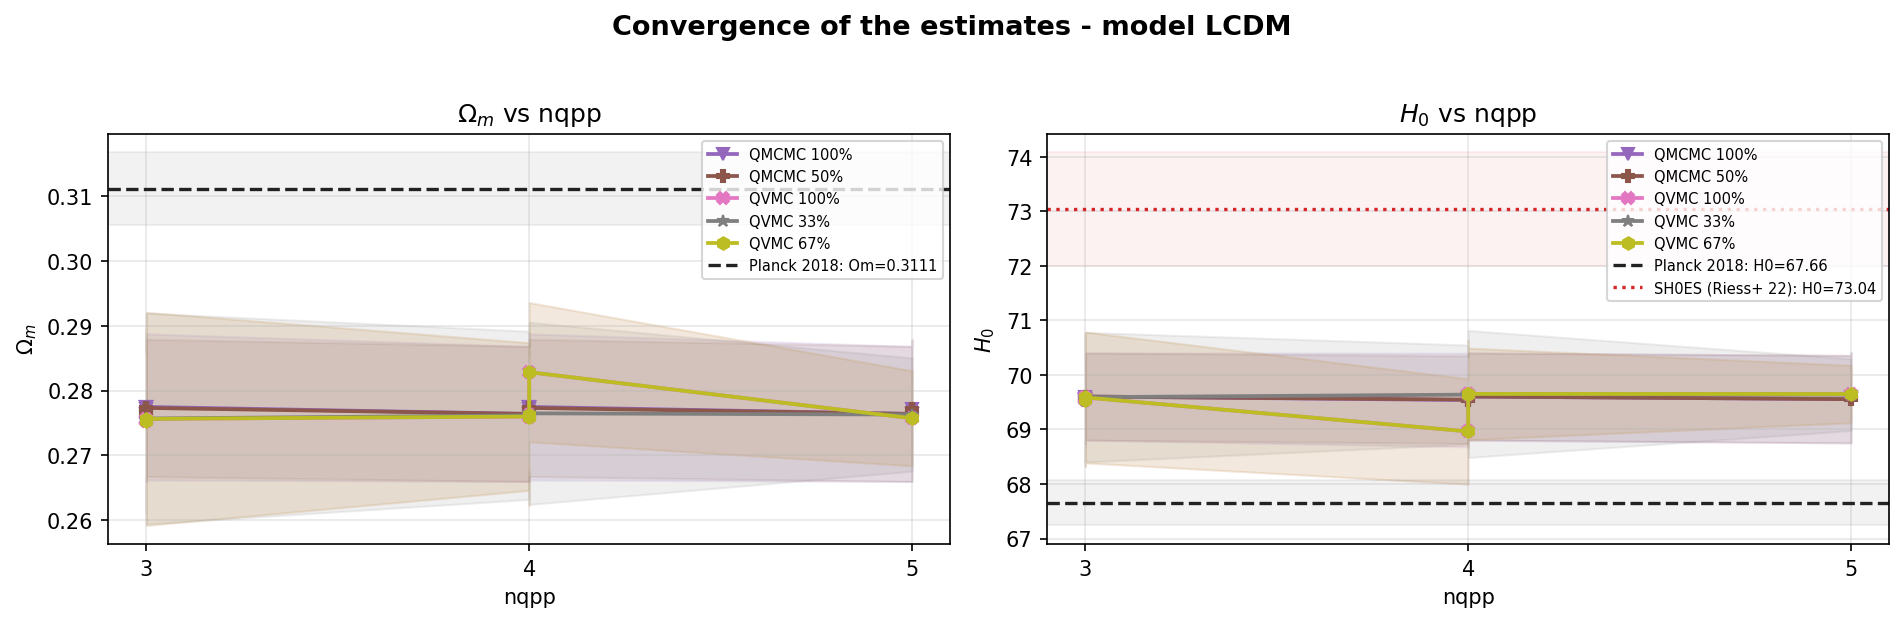
\includegraphics[width=\textwidth]{figs/a_convergence.png}
\caption{$\Lambda$CDM. Las curvas son esencialmente planas entre
\texttt{nqpp}$=3$ y $5$: el resultado no depende del tamaño del registro. La
única que se mueve es QVMC $67\%$ (verde oliva) en \texttt{nqpp}$=4$, y vuelve
a la línea en $5$. Las bandas de $\pm\sigma$ se solapan por completo, así que
ese movimiento no es significativo.}
\end{figure}

\noindent
\textbf{Qué mirar primero:} si una curva \emph{sí} tiene pendiente, el
resultado depende de una elección de implementación y no sólo de los datos.
Eso hay que reportarlo, no promediarlo.

% ---------------------------------------------------------------------
\subsection{\texttt{cost\_<modelo>} --- qué cuesta cada peldaño}
\archivo{cost\_lcdm.\{png,pdf\}}

Tiempo de pared contra \texttt{nqpp}, una curva por método.

\contesta{Cuánto cuesta cada método \textbf{en el simulador}. Nada más.}

\begin{figure}[H]
\centering
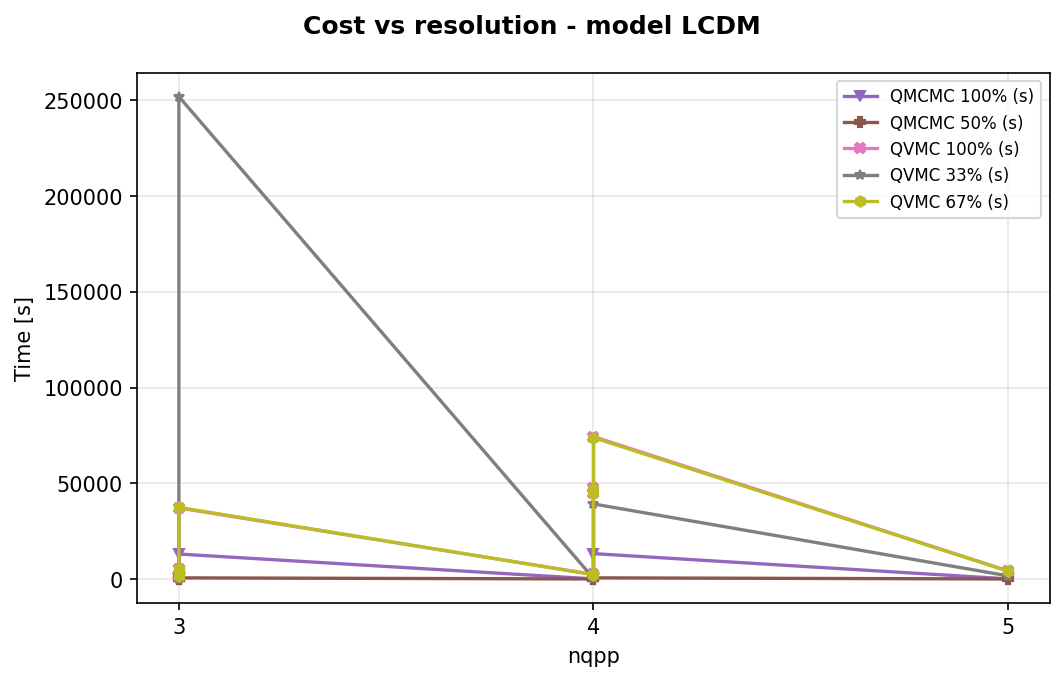
\includegraphics[width=.86\textwidth]{figs/b_cost.png}
\caption{$\Lambda$CDM. Los dos peldaños del QMCMC (morado y café) están
pegados al eje; los del QVMC suben tres órdenes de magnitud. Esta figura mide
\textbf{Aer}, no hardware cuántico: no sostiene ninguna afirmación sobre
velocidad real.}
\end{figure}

\noindent
\Al{Limitación conocida.} Esta figura \textbf{junta todos los niveles de
ruido} en una sola curva por método. Por eso una curva puede bajar al crecer
\texttt{nqpp}: no es que el problema se abarate, es que los puntos de la
derecha vienen de celdas sin ruido y los de la izquierda de celdas ruidosas.
Léela como un orden de magnitud. Para el tiempo celda por celda, usa el panel
de tiempo de \texttt{ruido\_fijo\_*} o la columna \texttt{Time\_s} del CSV,
que sí separan por nivel de ruido.

% ---------------------------------------------------------------------
\subsection{\texttt{convergence\_<modelo>\_genetico} --- la rejilla del genético}
\archivo{convergence\_lcdm\_genetico.\{png,pdf\}}

Lo mismo que arriba pero con eje $x$ = \texttt{n\_bits} y sólo los métodos
genéticos.

\contesta{¿Cuántos bits por gen hacen falta para que el genético deje de
depender de la codificación?}

\begin{figure}[H]
\centering
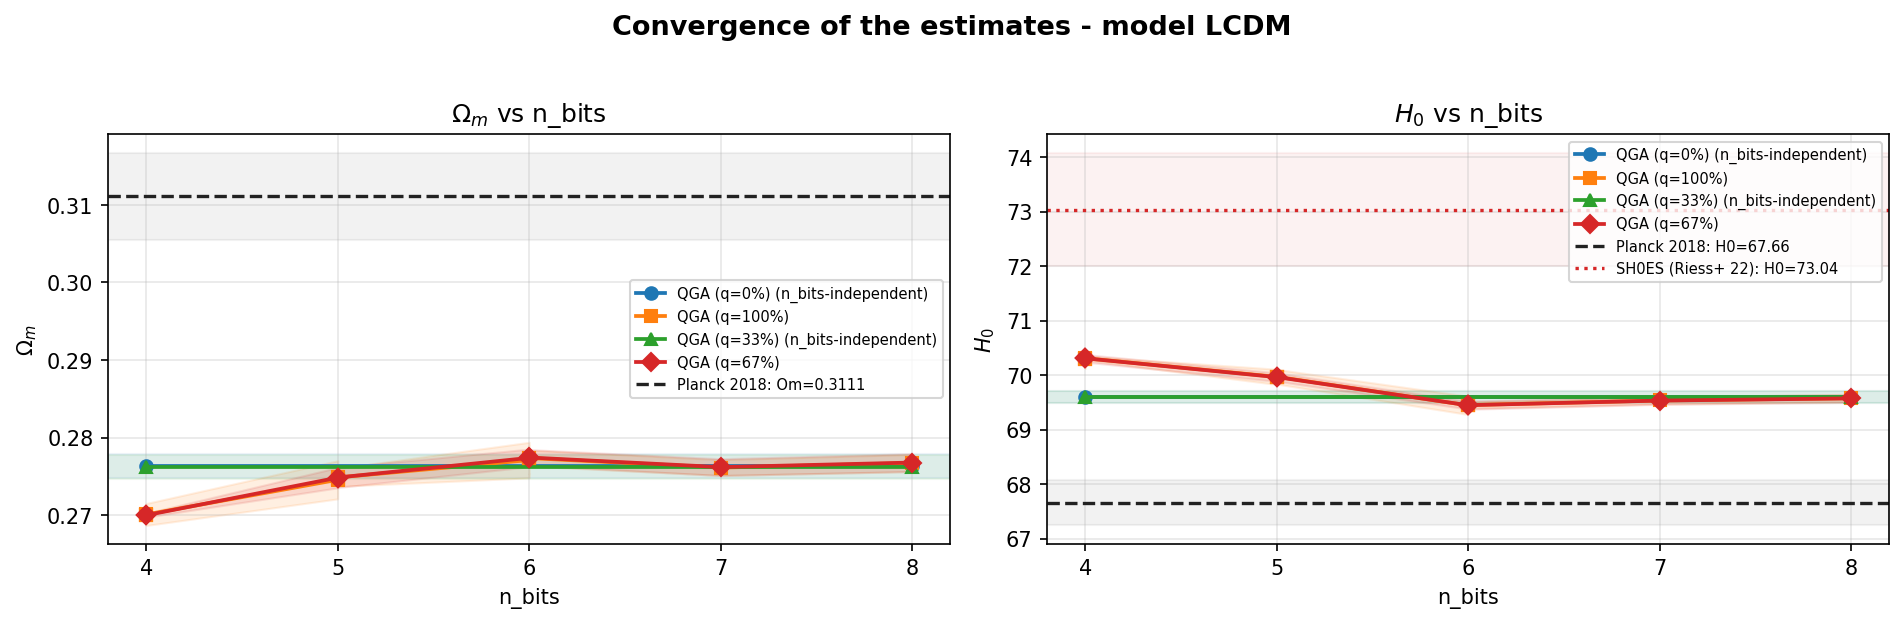
\includegraphics[width=\textwidth]{figs/q_convergence_gen.png}
\caption{$\Lambda$CDM. QGA $67\%$ (rojo) arranca en $\Omega_m = 0.270$ con
\texttt{n\_bits}$=4$ y converge a $0.2765$ a partir de $6$. Los peldaños de
$0\%$ y $33\%$ salen marcados como \emph{n\_bits-independent}: no dependen de
la codificación porque sus operadores no la tocan. \textbf{La lectura es que
con 4 bits la rejilla es demasiado gruesa} y por debajo de 6 no conviene
reportar.}
\end{figure}

% ---------------------------------------------------------------------
\subsection{\texttt{cost\_<modelo>\_genetico}}
\archivo{cost\_lcdm\_genetico.\{png,pdf\}}

\contesta{Dónde se vuelve impagable el genético cuántico.}

\begin{figure}[H]
\centering
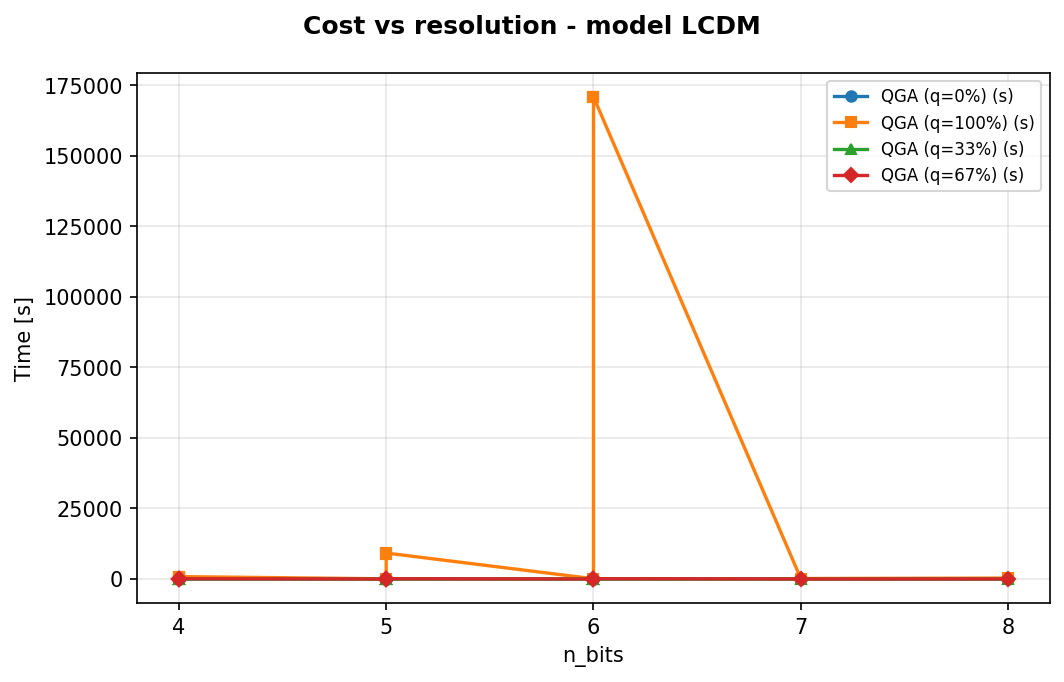
\includegraphics[width=.8\textwidth]{figs/r_cost_gen.png}
\caption{El peldaño de $100\%$ es el que dispara el costo, porque el operador
de cruce usa $2\,n_b$ qubits y con matriz de densidad eso crece muy rápido.
Es la razón por la que el QGA $100\%$ con ruido es inviable a partir de
$n_b = 6$.}
\end{figure}

% =====================================================================
\clearpage
\section{Por tarea: la escalera de quantumness}
% =====================================================================

Viven dentro de la carpeta de cada tarea de samplers. Se rehacen con la
opción \texttt{-{}-replot-ladder} del módulo principal.

% ---------------------------------------------------------------------
\subsection{\texttt{ladder\_trends\_<modelo>} --- la figura central del marco}
\archivo{ladder\_trends\_lcdm.\{png,pdf\}}

Rejilla de 8 a 10 paneles. Eje $x$: porcentaje de quantumness ($0 \to 100$),
un punto por peldaño. Rojo = QMCMC, naranja = QVMC. Un panel por parámetro
cosmológico, más runtime, $\chi^2_\nu$, AIC, BIC, ESS y aceptación/KL.

\contesta{Qué cambia, y sobre todo qué \emph{no} cambia, al ir encendiendo
componentes cuánticos.}

\begin{figure}[H]
\centering
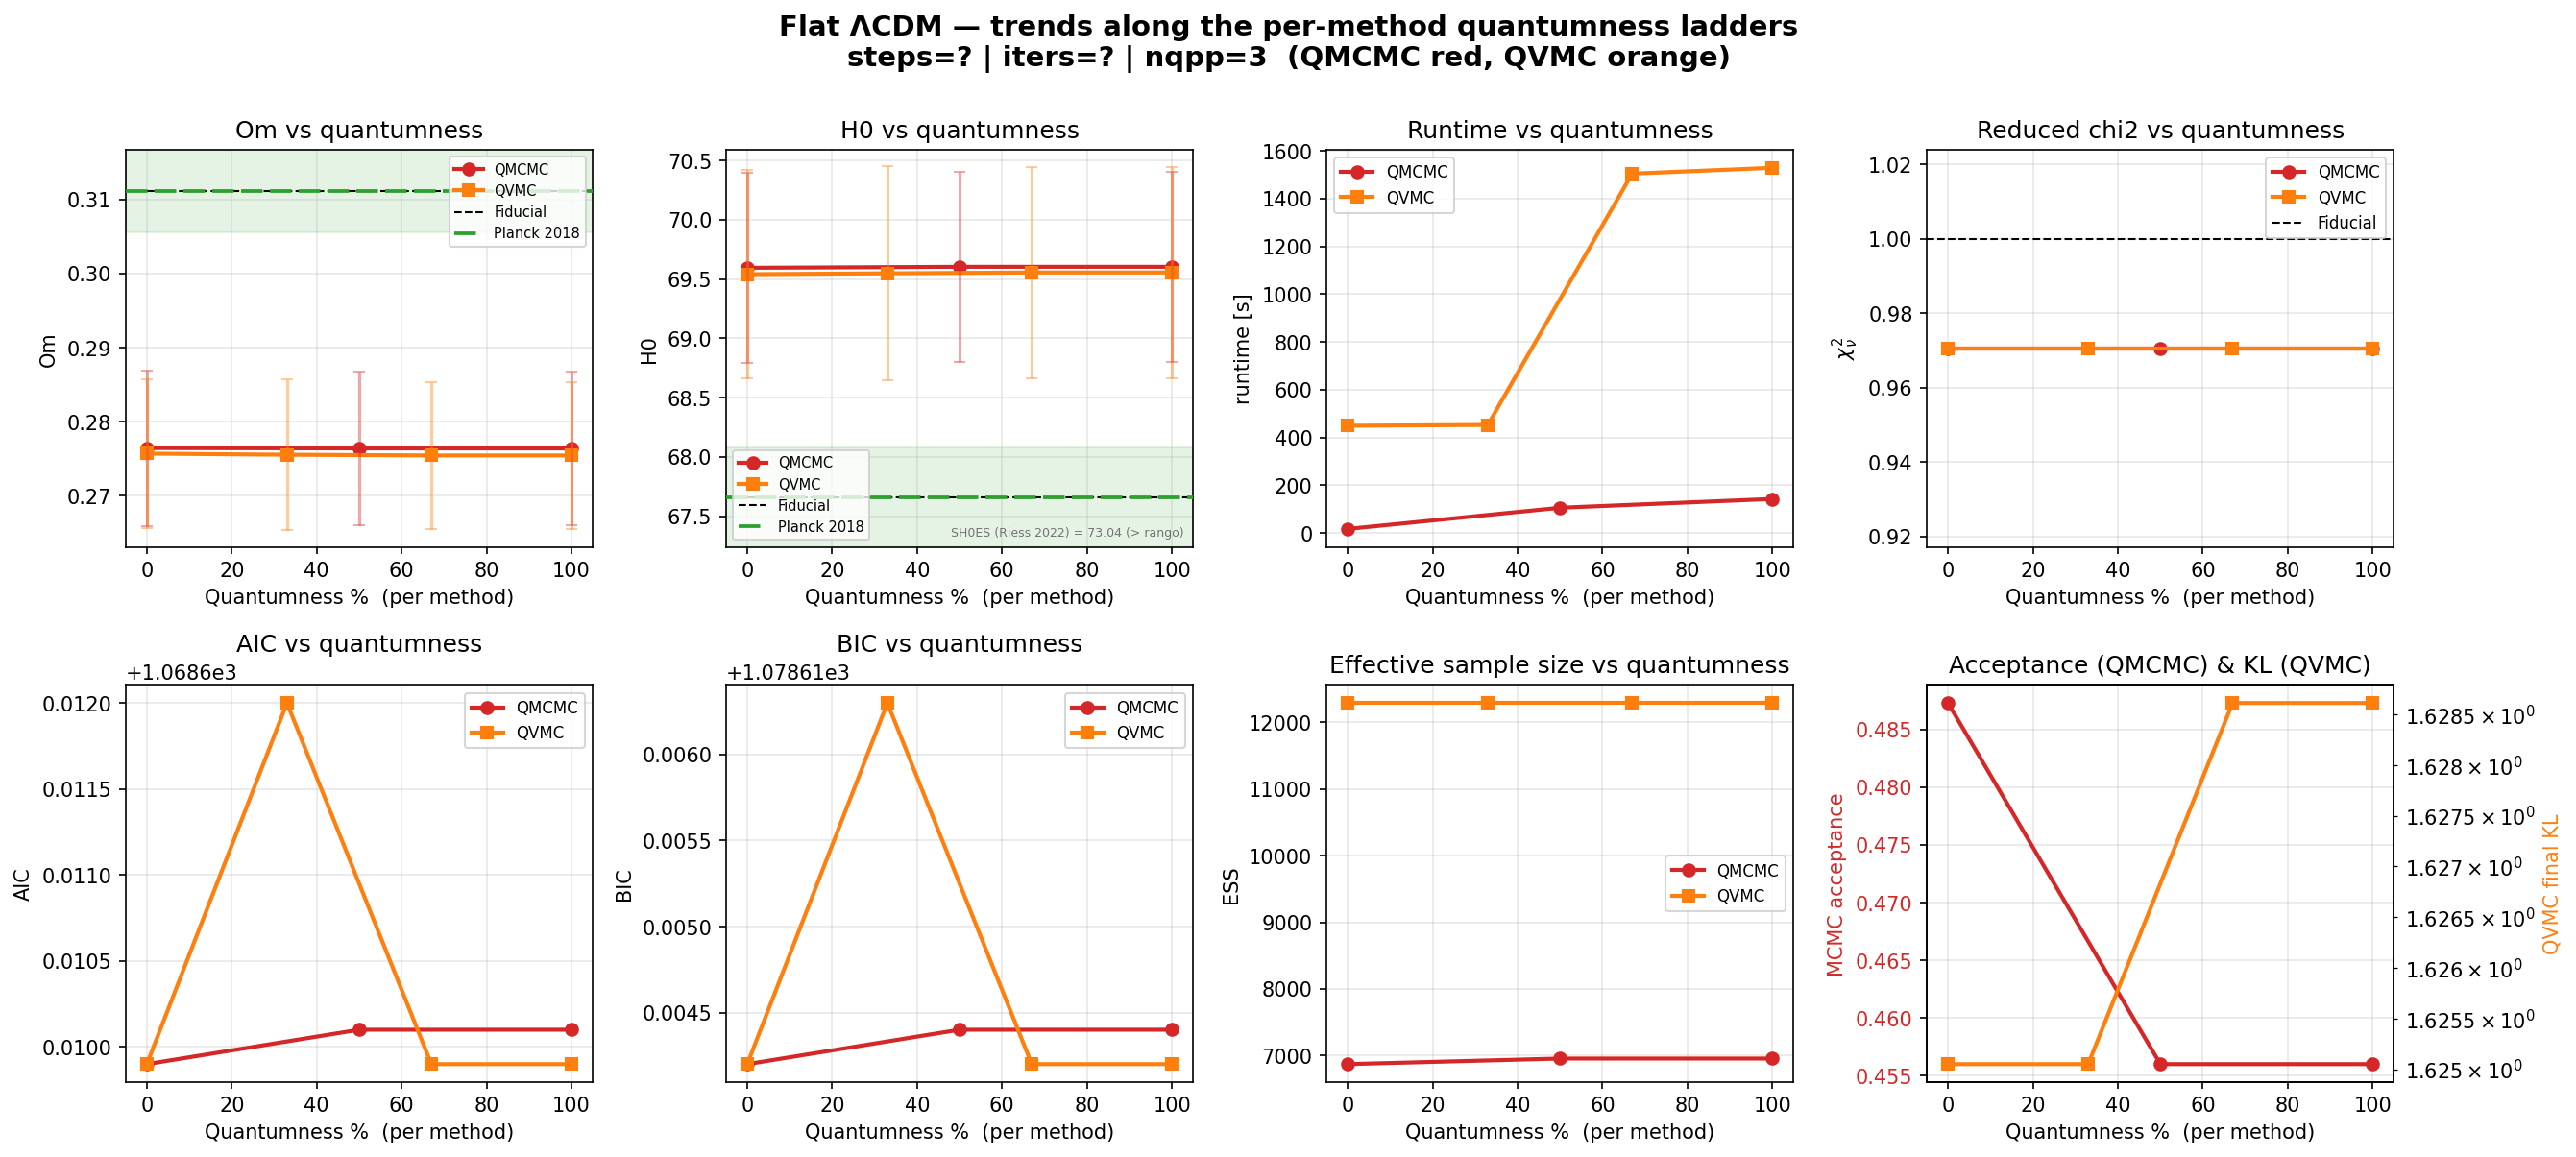
\includegraphics[width=\textwidth]{figs/c_ladder_trends.png}
\caption{$\Lambda$CDM, \texttt{nqpp}$=3$. En los paneles de $\Omega_m$ y $H_0$
las dos series son \textbf{líneas planas}: encender componentes cuánticos no
mueve los parámetros. Eso es exactamente la afirmación de fidelidad. Lo que sí
cambia es el runtime, que salta de $\sim 450$ a $\sim 1500$ segundos entre el
$33\%$ y el $67\%$ del QVMC.}
\end{figure}

\noindent
\textbf{Qué mirar primero:} los paneles de parámetros. Plano es el resultado
deseado. Si se inclinan, la quantumness está cambiando la física, que es
justo lo que el marco existe para detectar.

% ---------------------------------------------------------------------
\subsection{\texttt{ladder\_summary\_<modelo>} --- los mismos números, en tabla}
\archivo{ladder\_summary\_lcdm.\{png,pdf\}}

\contesta{Los valores exactos, para citarlos sin tener que leerlos de una
gráfica.}

\begin{figure}[H]
\centering
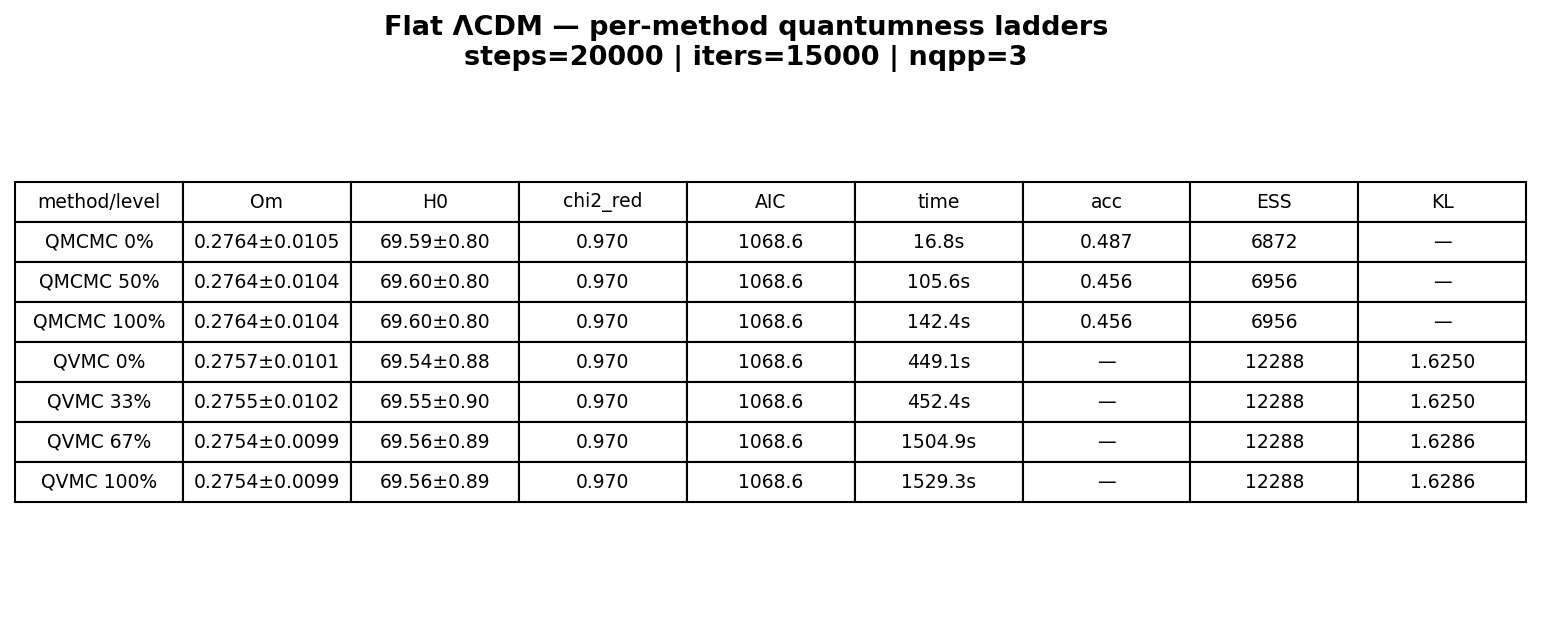
\includegraphics[width=\textwidth]{figs/d_ladder_summary.png}
\caption{Aquí se ven de golpe las dos parejas fieles: QMCMC $50\%$ y $100\%$
dan $0.2764 \pm 0.0104$ \emph{idéntico}, y QVMC $67\%$ y $100\%$ dan
$0.2754 \pm 0.0099$ idéntico. También se ve que el ESS del variacional es
$12288$ en los cuatro peldaños: \textbf{ahí el ESS es el número de disparos,
no una medida de calidad}, y por eso no se compara entre familias.}
\end{figure}

% ---------------------------------------------------------------------
\subsection{\texttt{ladder\_rhat\_qmcmc\_<modelo>} --- ¿convergió la cadena?}
\archivo{ladder\_rhat\_qmcmc\_lcdm.\{png,pdf\}}

$\hat{R} - 1$ contra pasos de muestreo, eje $y$ logarítmico, una curva por
peldaño. La línea punteada es el umbral $\hat{R} - 1 = 0.01$.

\contesta{¿Convergió la cadena, y convergió igual de rápido en todos los
peldaños?}

\begin{figure}[H]
\centering
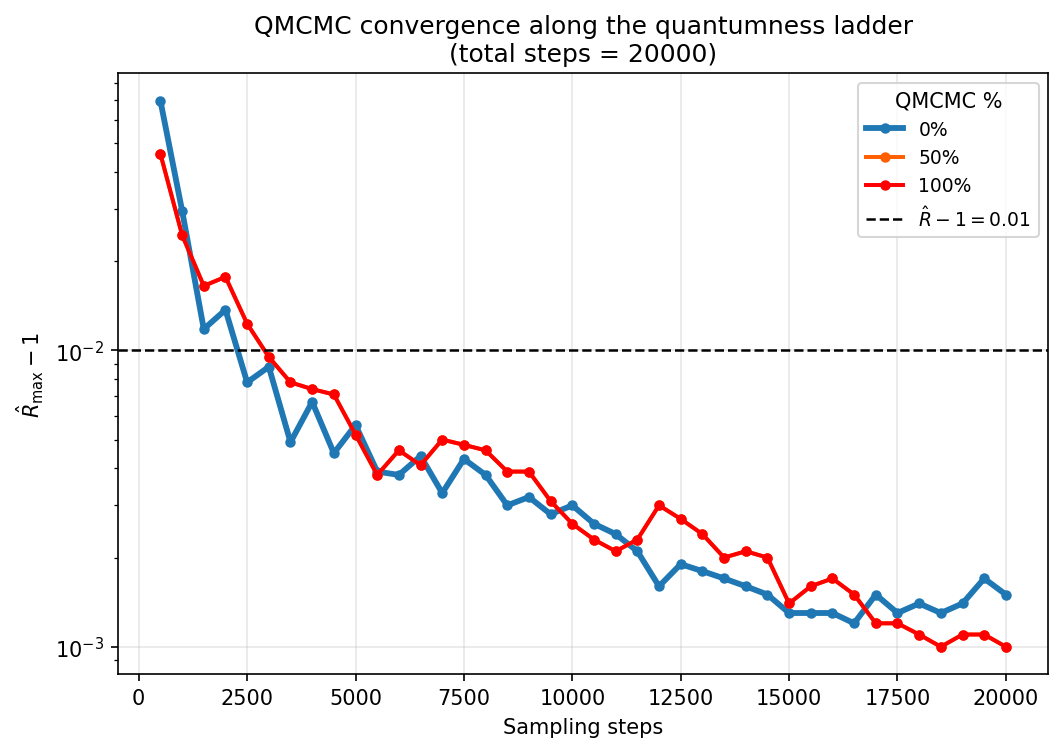
\includegraphics[width=.72\textwidth]{figs/e_ladder_rhat.png}
\caption{Las dos curvas cruzan el umbral cerca de los $2500$--$3000$ pasos y
terminan en $\hat{R} - 1 \approx 10^{-3}$, muy por debajo del criterio. El
peldaño cuántico (rojo) tarda un poco más en cruzar pero acaba igual. Que las
dos curvas se persigan sin separarse es otra forma de ver la fidelidad.}
\end{figure}

\noindent
\Al{Criterio duro:} si una curva no baja del umbral, esa celda \textbf{no es
citable}. No se sabe siquiera si la lista de puntos es una muestra de la
posterior, y entonces la barra de error no significa nada.

% ---------------------------------------------------------------------
\subsection{\texttt{ladder\_kl\_qvmc\_<modelo>} --- el techo del ansatz}
\archivo{ladder\_kl\_qvmc\_cpl.\{png,pdf\}}

KL contra iteración de entrenamiento, \textbf{logarítmico en los dos ejes}.

\contesta{(1) ¿A qué valor se estanca el entrenamiento? (2) ¿Cuántas
iteraciones gastó cada peldaño?}

\begin{figure}[H]
\centering
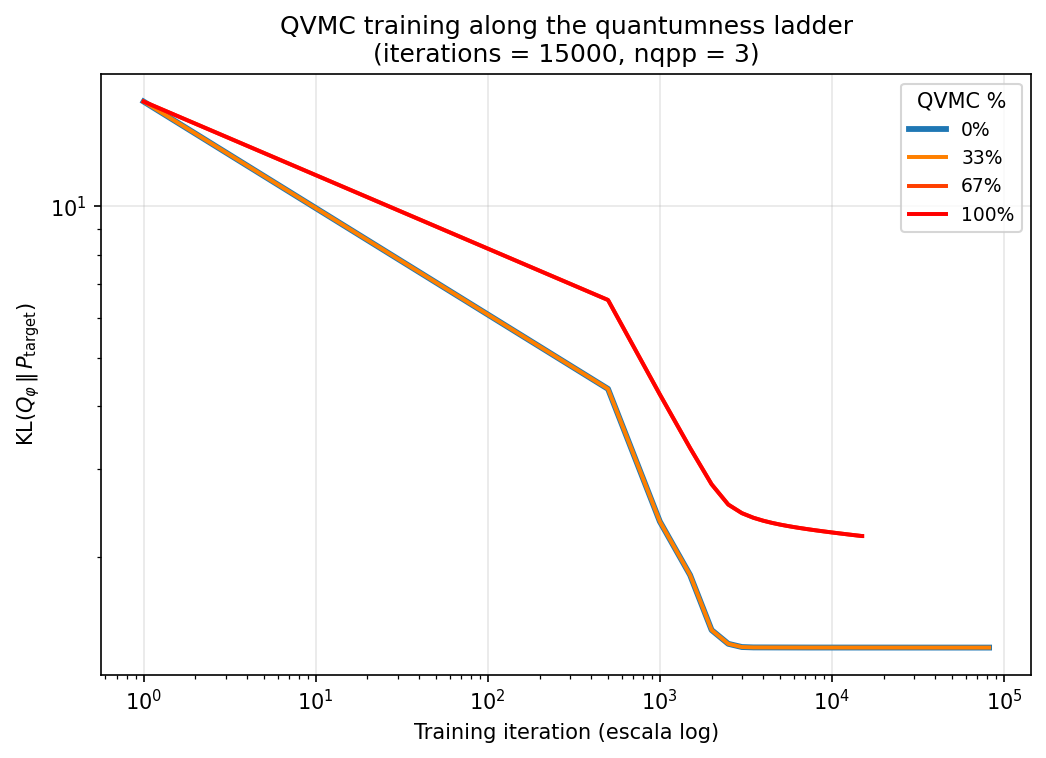
\includegraphics[width=.8\textwidth]{figs/f_ladder_kl.png}
\caption{CPL, \texttt{nqpp}$=3$. Las cuatro curvas bajan y se aplanan. Ese
piso \textbf{es el techo de expresividad del ansatz}: con $n(2L+1) = 7n$
ángulos contra $2^n - 1$ grados de libertad, la KL no puede llegar a cero y
no hay que esperar que lo haga. No es un fallo de convergencia.}
\end{figure}

\noindent
\textbf{Y aquí hay algo que sí hay que explicar en el paper.} Los peldaños
\textbf{no gastan el mismo número de iteraciones}: el de $33\%$ llega a
$\sim 10^5$ mientras los de $67\%$ y $100\%$ paran en $1.5\times 10^4$. No es
un error. El presupuesto se iguala por \textbf{circuitos}, no por iteraciones,
y el optimizador clásico de \texttt{scipy} cuenta evaluaciones de función.
Con eje lineal el peldaño más largo se comía toda la escala y los otros tres
quedaban aplastados contra el margen izquierdo, que es justo donde ocurre la
bajada que interesa; en log se ven los cuatro y la diferencia de presupuesto
queda a la vista. No se recorta ni un punto (marcador \texttt{[B-KLLOGX]}).

% ---------------------------------------------------------------------
\subsection{\texttt{corner\_ladder\_<familia>\_<modelo>} --- la prueba visual}
\archivo{corner\_ladder\_qmcmc\_lcdm.\{png,pdf\}}

Contornos 2D de la posterior con las marginales 1D, un color por peldaño.

\contesta{¿La posterior cuántica es la misma que la clásica? A ojo, de un
vistazo.}

\begin{figure}[H]
\centering
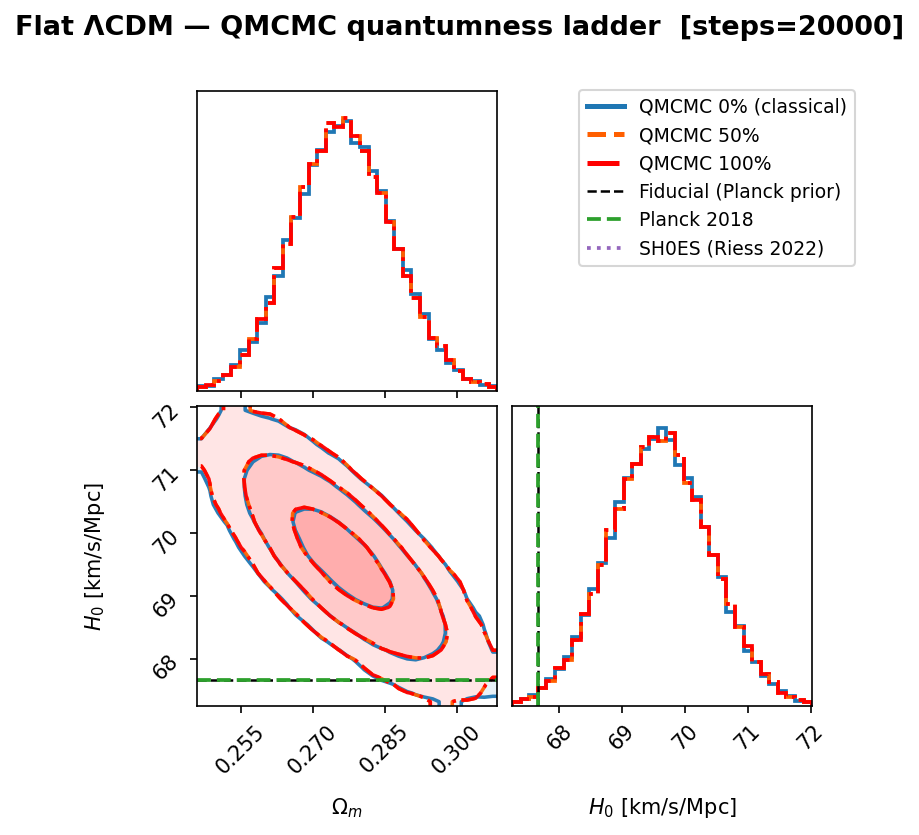
\includegraphics[width=.66\textwidth]{figs/g_corner_ladder.png}
\caption{$\Lambda$CDM. Los tres peldaños ---$0\%$ clásico, $50\%$ y $100\%$---
\textbf{caen uno encima del otro}, tanto en los contornos como en las
marginales. Es la fidelidad vista directamente, sin pasar por ningún número
resumido. Ésta es probablemente la figura más convincente del proyecto para
una presentación.}
\end{figure}

\noindent
\Al{No se pueden rehacer.} Los \texttt{corner} necesitan las \emph{cadenas}, y
las cadenas no se guardan en el CSV. Las que existen son las de la corrida
original: si se pierde la carpeta, hay que volver a correr.

% ---------------------------------------------------------------------
\subsection{\texttt{corner\_ladder\_1to1\_*} --- peldaño contra peldaño}
\archivo{corner\_ladder\_1to1\_qvmc\_lcdm\_q100.\{png,pdf\}}

El mismo corner pero de a dos: un peldaño cuántico contra su referencia
clásica.

\contesta{Cuando en el corner completo se encima todo, ¿cuál es exactamente
la discrepancia de \emph{este} peldaño?}

\begin{figure}[H]
\centering
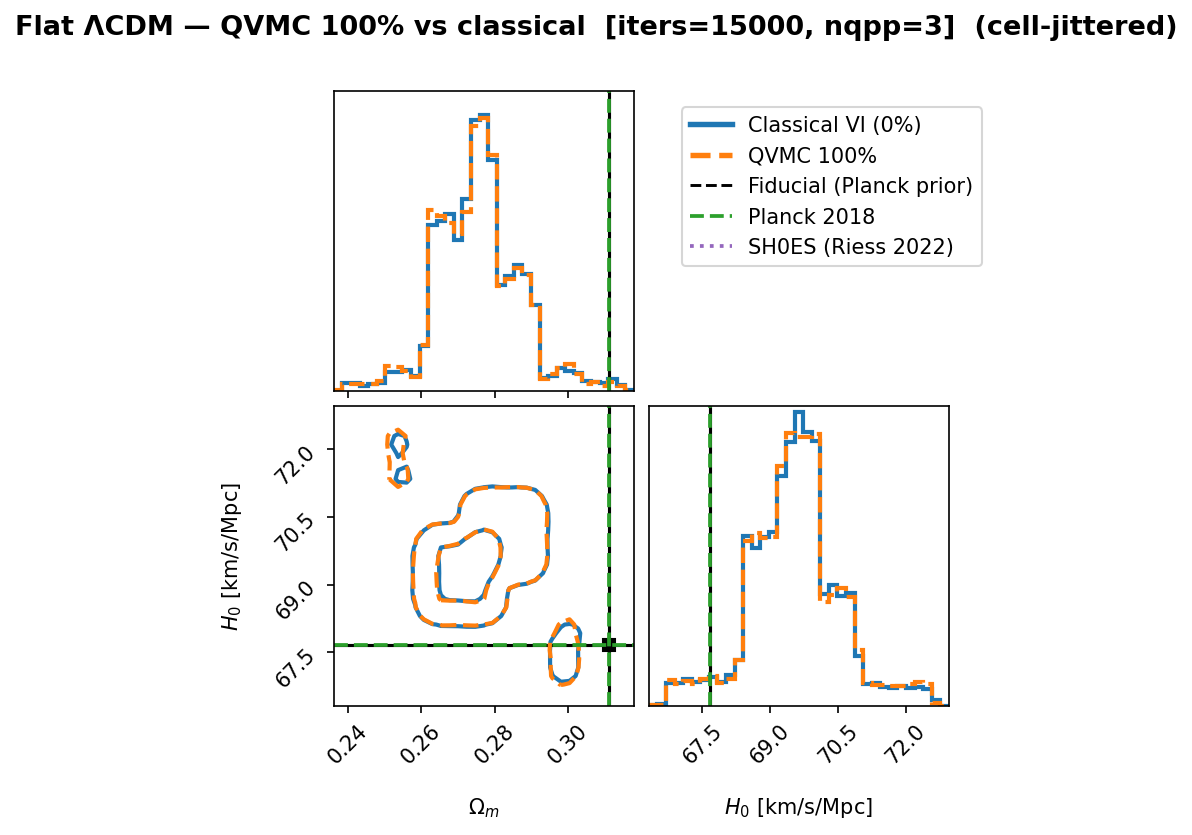
\includegraphics[width=.6\textwidth]{figs/h_corner_1to1.png}
\caption{QVMC $100\%$ contra el clásico. Aquí es donde se ve la
sub-dispersión del variacional: los contornos cuánticos son \emph{más
angostos}. Por eso esta figura acompaña bien a
\texttt{incertidumbre\_reportada}.}
\end{figure}

% =====================================================================
\clearpage
\section{Por tarea: los genéticos}
% =====================================================================

Viven dentro de \texttt{genetic\_*/model\_*/}.

% ---------------------------------------------------------------------
\subsection{\texttt{fitness\_<modelo>\_fitness}}
\archivo{fitness\_lcdm\_fitness.\{png,pdf\}}

Mejor $\chi^2$ de la población contra generación, una curva por peldaño.

\contesta{¿Se estancó el genético, y en qué valor acabó cada peldaño?}

\begin{figure}[H]
\centering
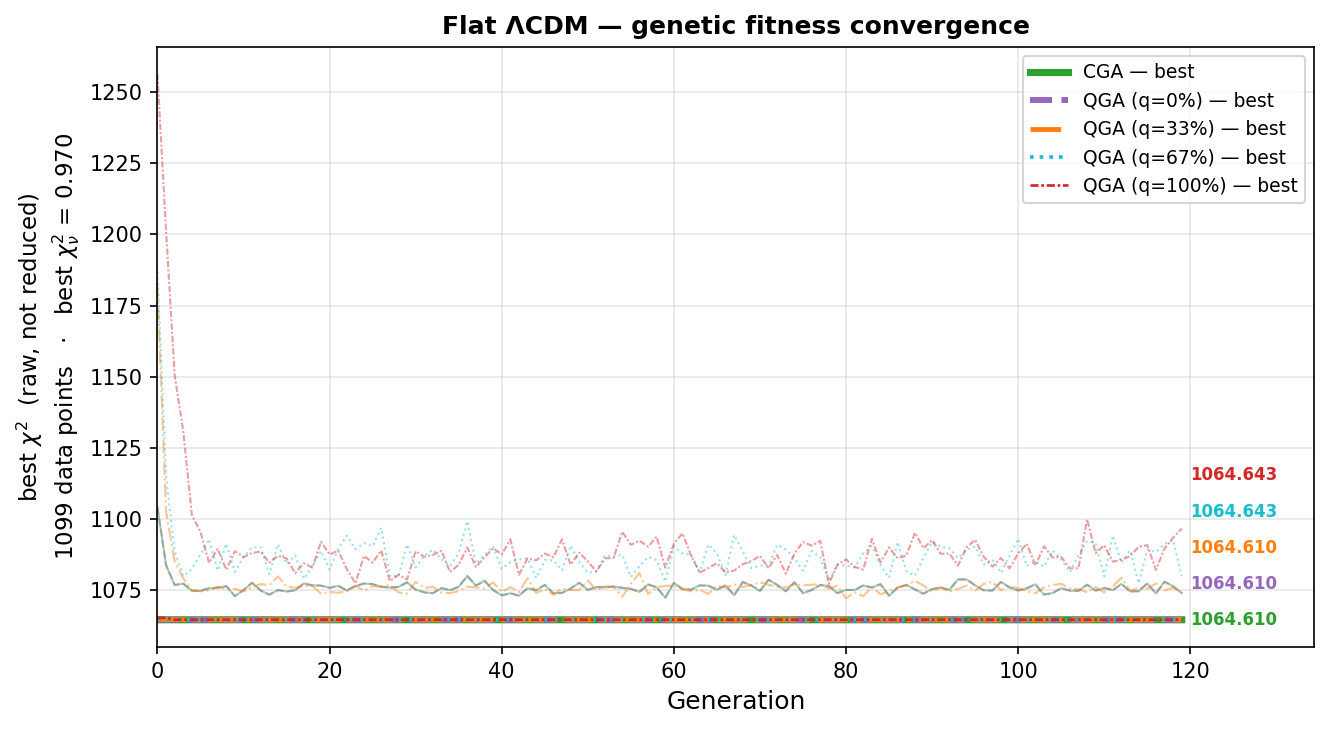
\includegraphics[width=.86\textwidth]{figs/i_fitness.png}
\caption{$\Lambda$CDM, $n_b = 6$. Todo el descenso ocurre en las primeras
$\sim 5$ generaciones; las $115$ restantes sólo fluctúan. Los valores finales
están anotados a la derecha: CGA, QGA $0\%$ y QGA $33\%$ terminan en
$1064.610$ y los de $67\%$ y $100\%$ en $1064.643$ --- una diferencia de
$0.033$ en $\chi^2$, treinta veces por debajo del umbral de relevancia
$\Delta\chi^2 = 1$.}
\end{figure}

\noindent
\textbf{Detalle importante:} las curvas gruesas de arriba son el \emph{mejor
de la población generación a generación}, y las líneas planas de abajo son el
\emph{mejor histórico}. No son lo mismo; el resultado reportado es el segundo.

% ---------------------------------------------------------------------
\subsection{\texttt{genetic\_convergence\_<modelo>}}
\archivo{genetic\_convergence\_lcdm\_genetic\_convergence.\{png,pdf\}}

\contesta{Cómo se encoge la población alrededor del mejor individuo.}

\begin{figure}[H]
\centering
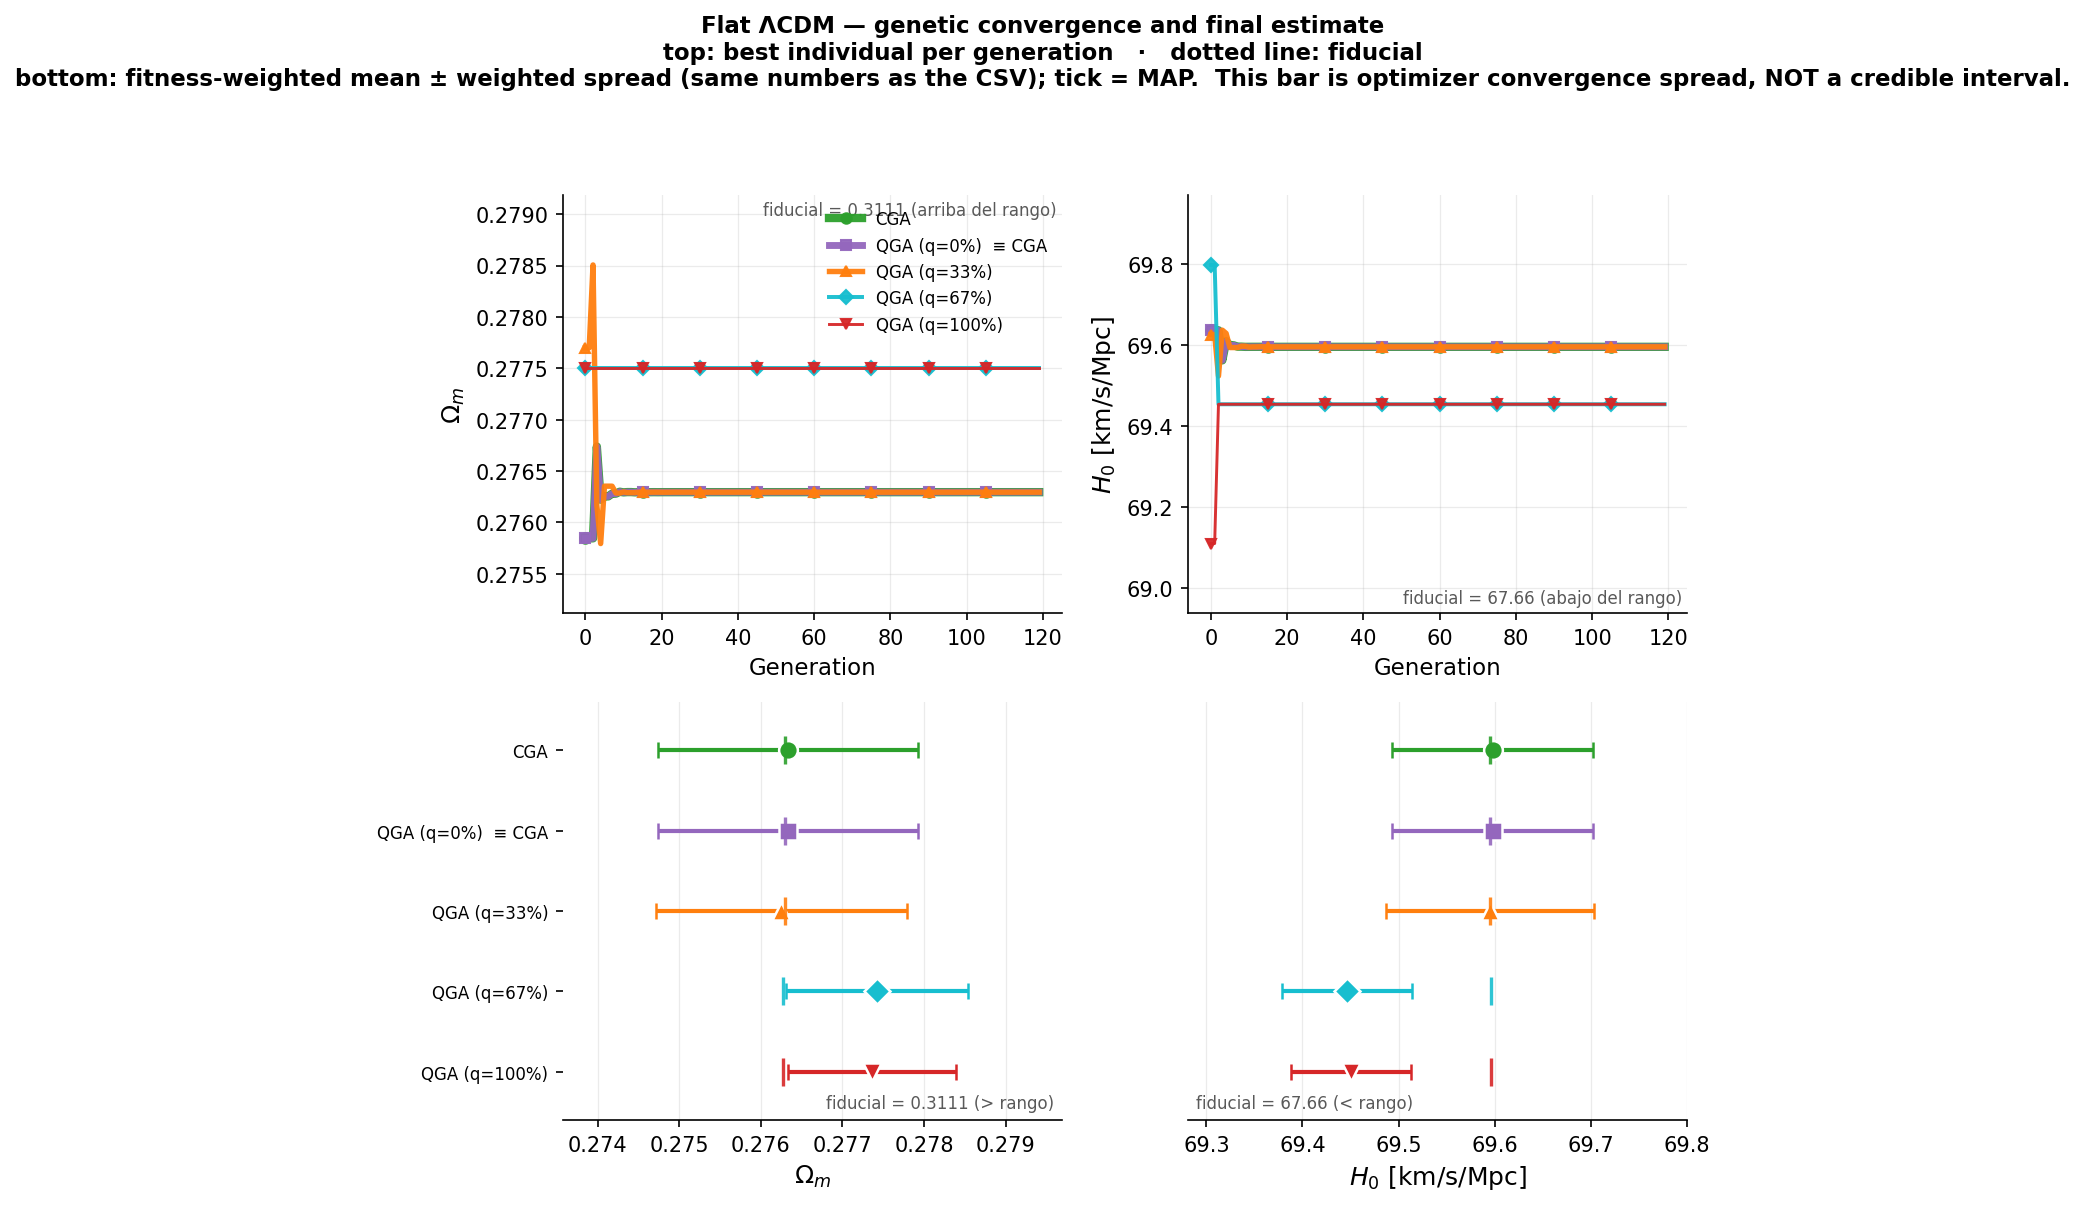
\includegraphics[width=.86\textwidth]{figs/j_genetic_conv.png}
\caption{Diagnóstico del optimizador. \Al{Cuidado:} la dispersión que se ve
aquí \textbf{no es una barra de error}. Un genético converge a un punto; que
la población se apriete no dice nada sobre cuánta incertidumbre tiene el
parámetro.}
\end{figure}

% =====================================================================
\clearpage
\section{El eje de ruido}
% =====================================================================

Viven en \texttt{figuras\_*/ruido\_*/}. Se generan con
\texttt{graficas\_ruido.py}. Son dos cortes de los mismos datos.

% ---------------------------------------------------------------------
\subsection{Las métricas, y qué cuenta como alarmante}

\begin{center}
\small
\begin{tabular}{@{}ll>{\raggedright\arraybackslash}p{6.4cm}@{}}
\toprule
\textbf{métrica} & \textbf{qué es} & \textbf{alarma} \\
\midrule
\texttt{desplazamiento} & $\max_p |\Delta p| / \sigma(\text{ideal})$
  & \Al{pasar de 1} \\
\texttt{acceptance} & fracción de pasos aceptados & que se desplome \\
\texttt{final\_KL} & KL al terminar el entrenamiento & que suba mucho \\
\texttt{chi2\_grid} & $\chi^2$ del mejor punto de rejilla, sin refinar & que suba \\
\texttt{Time\_s} & tiempo de pared & dónde está el salto \\
\bottomrule
\end{tabular}
\end{center}

\noindent
\textbf{Sólo el desplazamiento mide ciencia.} Las otras cuatro son
diagnósticos internos: pueden empeorar bastante sin que los parámetros se
muevan, y de hecho es lo que suele pasar. Un KL que sube al doble con ruido
no significa que el resultado cosmológico esté mal.

\medskip\noindent
\textbf{Las barras rayadas son \texttt{none-counts}}: el control \emph{sin}
ruido pero con el mismo número de disparos que las celdas ruidosas. Nunca
compares \texttt{none} contra un peldaño ruidoso sin mirar primero
\texttt{none-counts}: si no, estás confundiendo el efecto del ruido con el
del muestreo finito.

% ---------------------------------------------------------------------
\subsection{\texttt{ruido\_vs\_rejilla\_<familia>\_<modelo>\_<métrica>}}
\archivo{ruido\_vs\_rejilla\_samplers\_lcdm\_desplazamiento.\{png,pdf\}}

Un panel por método. Eje $x$: \texttt{nqpp} o \texttt{n\_bits}. Una curva por
peldaño de ruido.

\contesta{¿El daño del ruido \textbf{empeora} al crecer el registro?}

\begin{figure}[H]
\centering
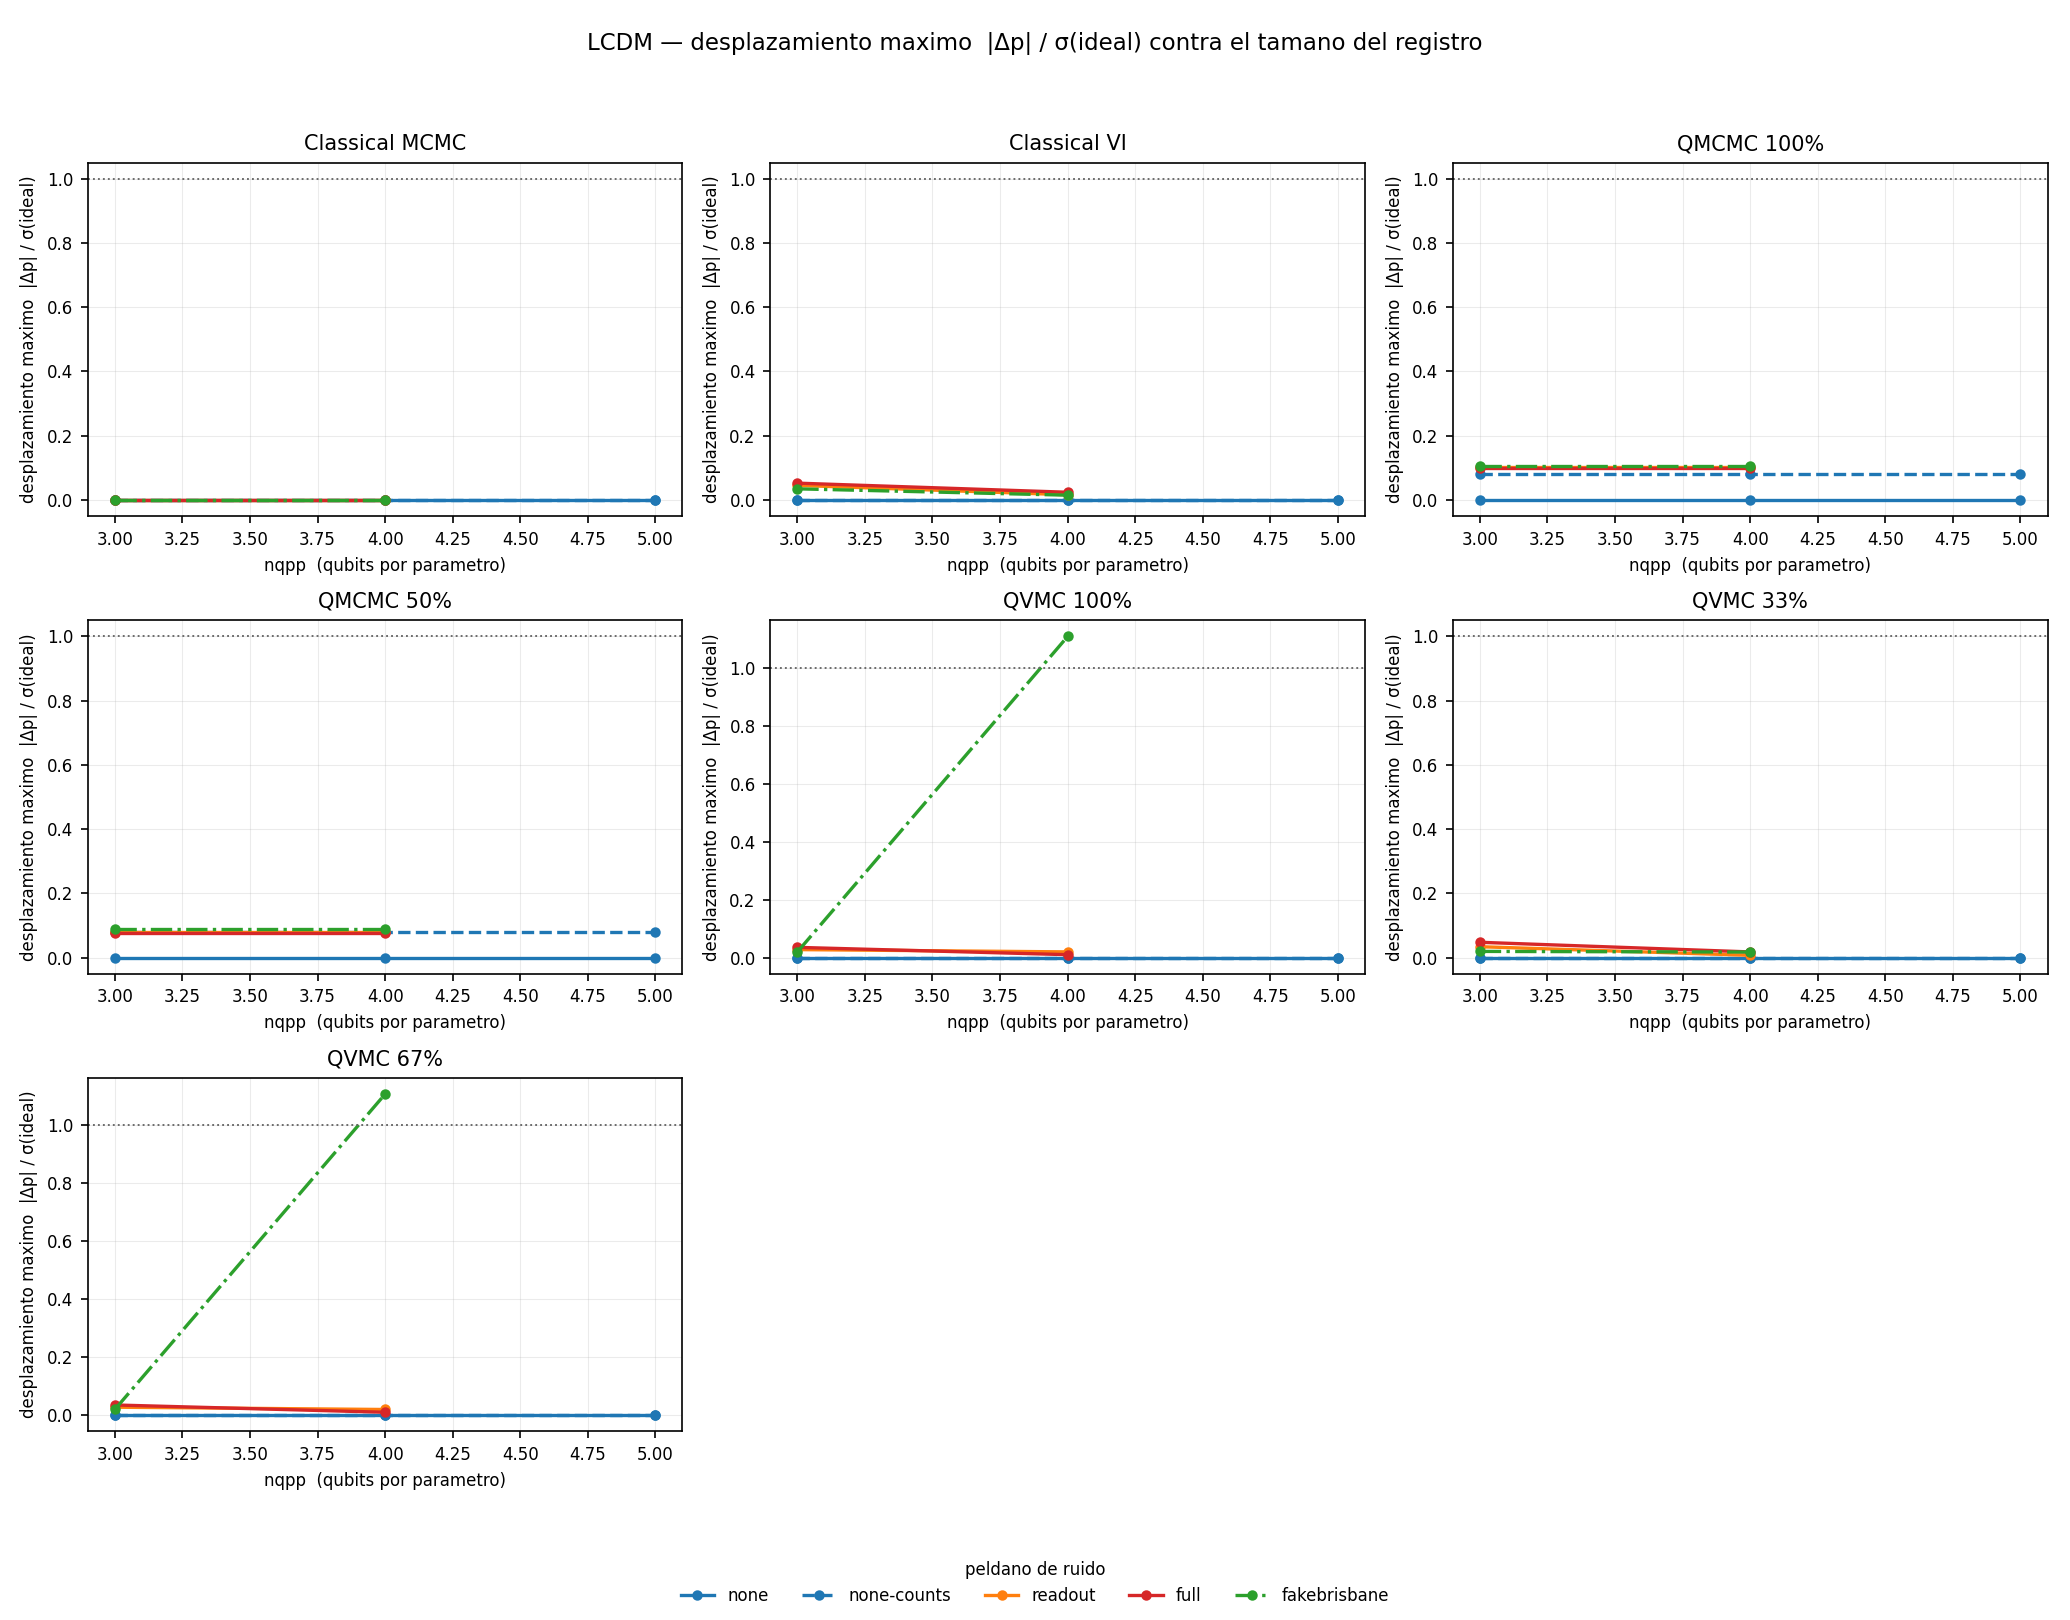
\includegraphics[width=\textwidth]{figs/k_ruido_vs_rejilla.png}
\caption{$\Lambda$CDM. Casi todo está pegado al cero. Las excepciones son
QVMC $67\%$ y $100\%$ bajo \texttt{FakeBrisbane} (verde), que suben con
pendiente fuerte y \textbf{cruzan la línea de $1\sigma$ en
\texttt{nqpp}$=4$}.}
\end{figure}

\noindent
Ésta es la figura que contesta la pregunta importante del eje de ruido. Una
curva ruidosa \emph{plana} pero desplazada es un sesgo fijo, molesto pero
acotado. Una curva ruidosa que \emph{se separa hacia la derecha} es mucho
peor: dice que el método se degrada conforme crece el registro, o sea que en
hardware real no escala. Es lo que está pasando con el QVMC bajo un backend
calibrado, y hay que decirlo.

% ---------------------------------------------------------------------
\subsection{\texttt{ruido\_fijo\_<familia>\_<modelo>\_<rejilla>}}
\archivo{ruido\_fijo\_samplers\_lcdm\_nqpp4.\{png,pdf\}}

Rejilla fija, los peldaños de ruido lado a lado, las cuatro métricas apiladas.

\contesta{En esta celda concreta, ¿qué cuesta el ruido, en cada cosa a la vez?}

\begin{figure}[H]
\centering
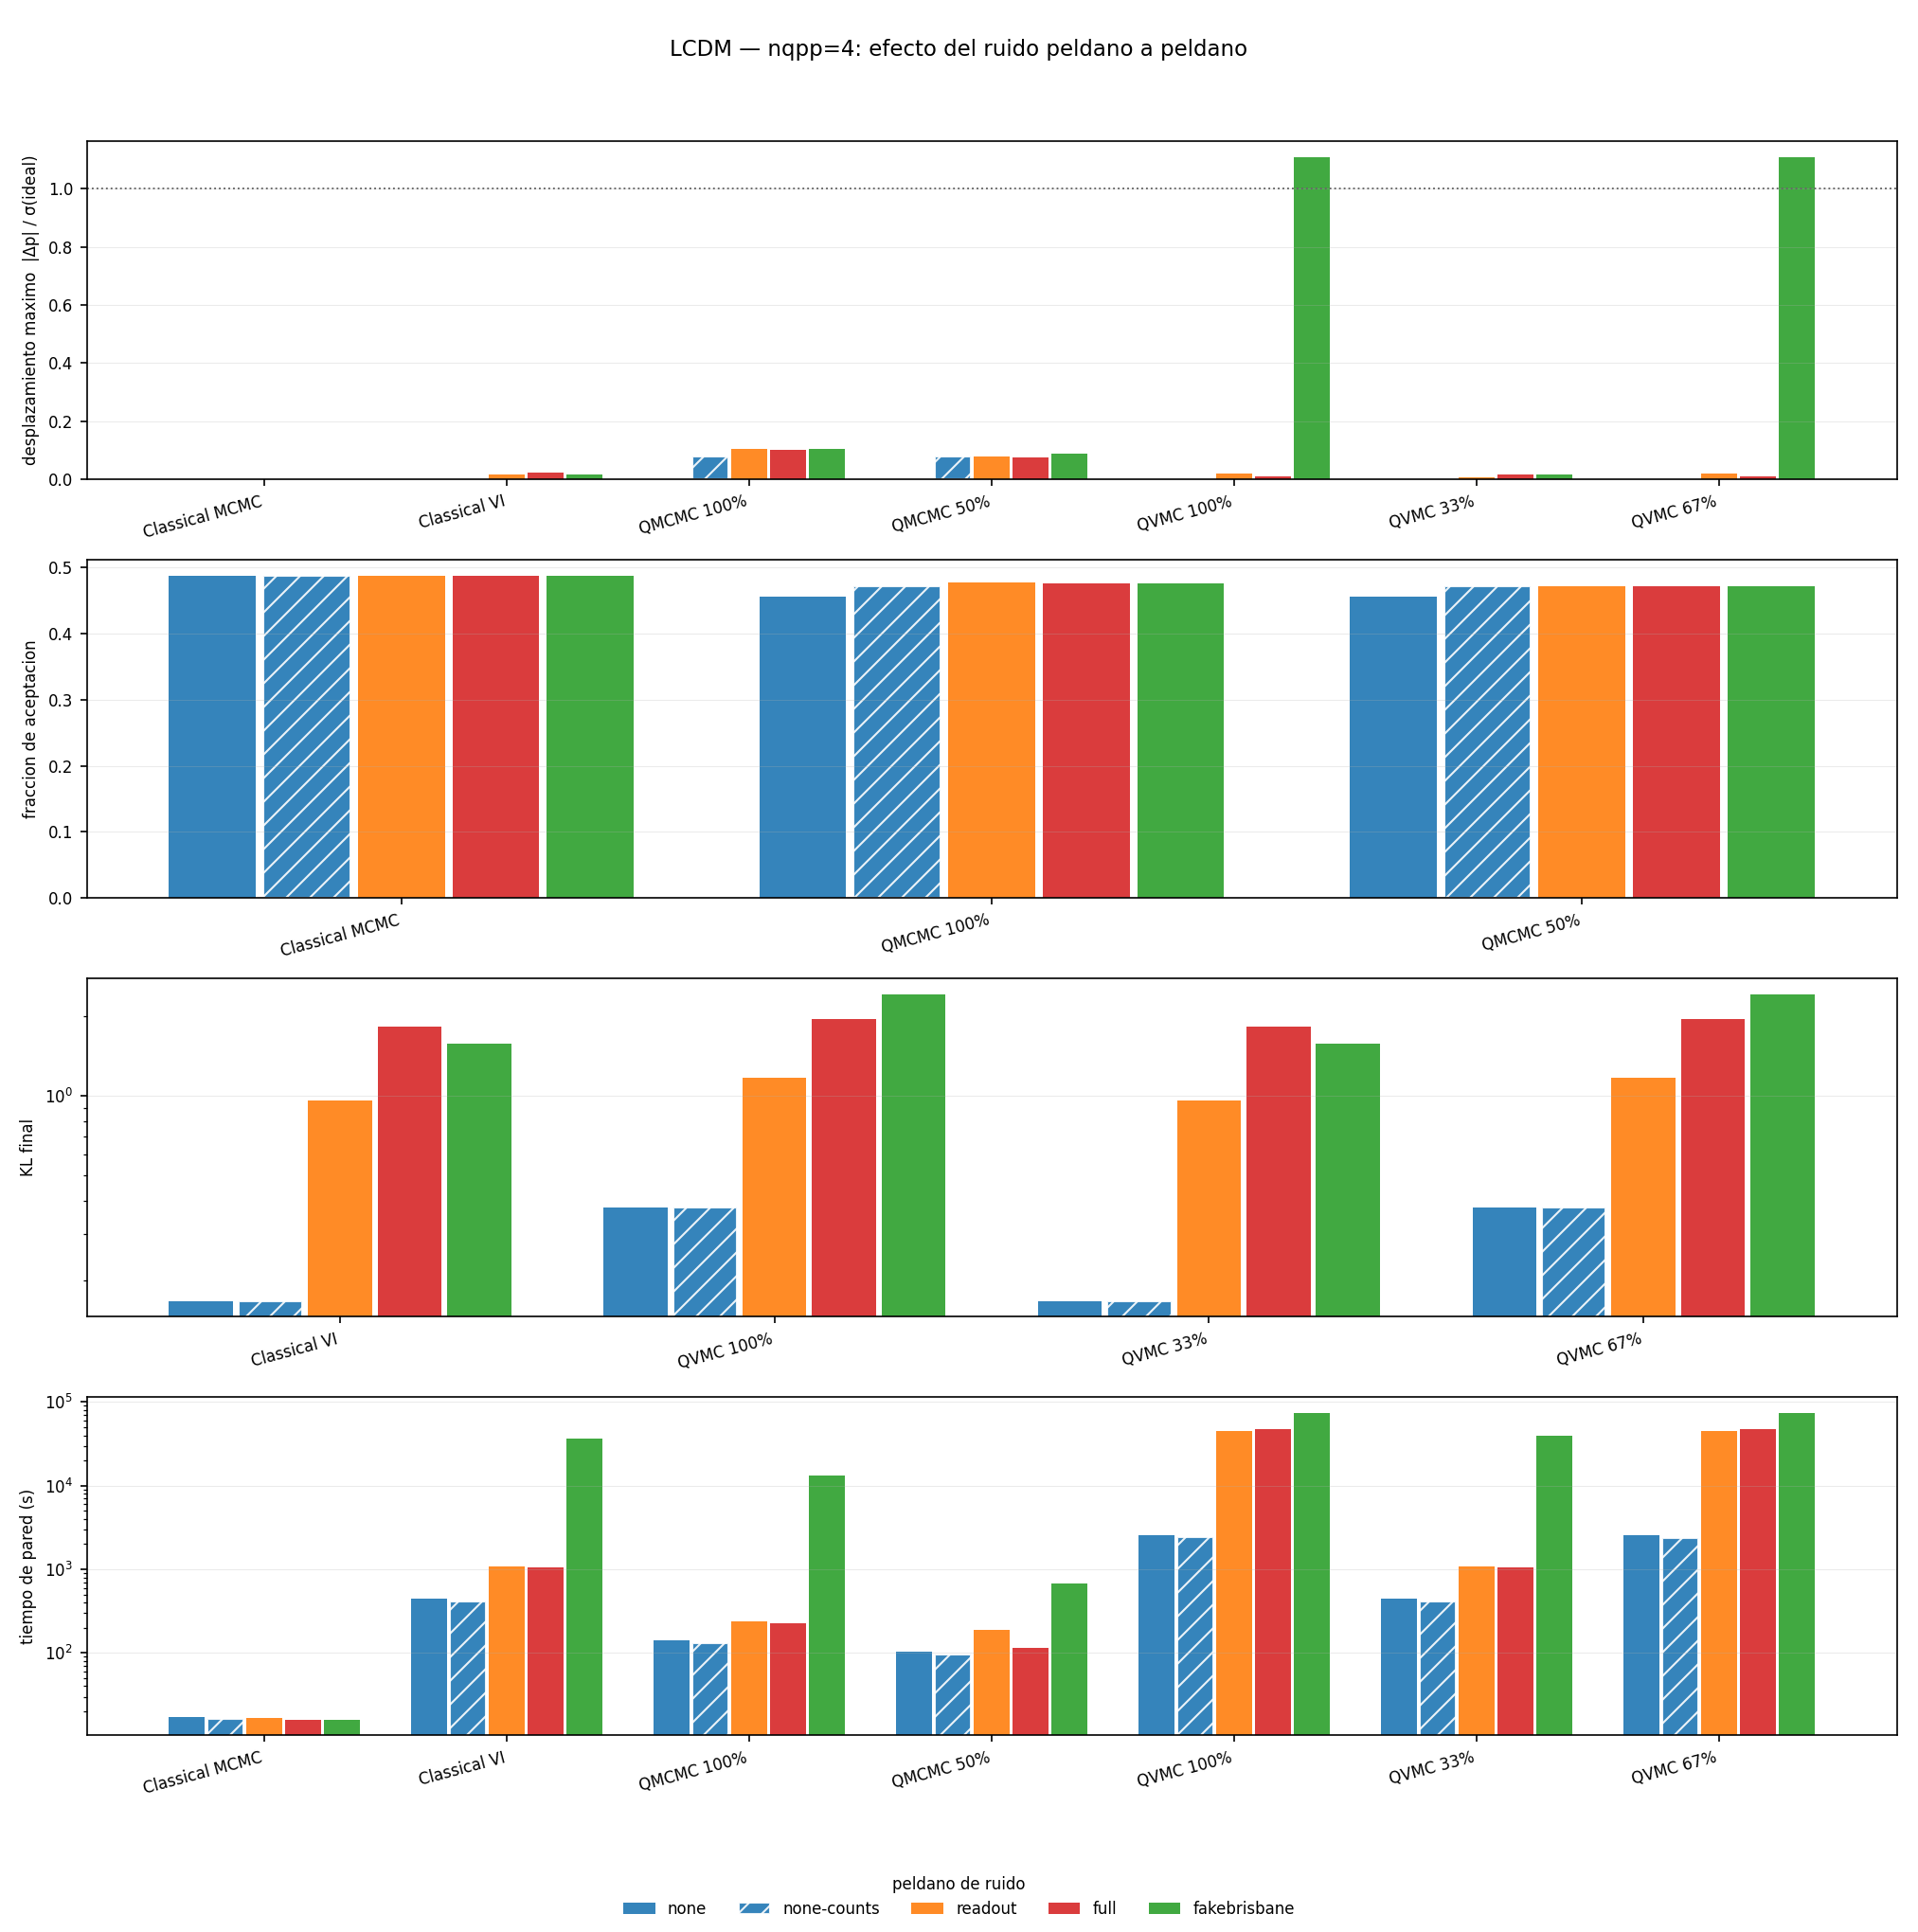
\includegraphics[width=.9\textwidth]{figs/l_ruido_fijo.png}
\caption{$\Lambda$CDM, \texttt{nqpp}$=4$. La lectura de conjunto es la
conclusión del eje entero: el desplazamiento está en el suelo salvo dos
barras verdes (QVMC $67\%$ y $100\%$ con \texttt{FakeBrisbane}, ambas por
encima de $1\sigma$); la aceptación es plana; el KL sube con el ruido; y el
tiempo sube muchísimo más --- de $10^2$ a $10^5$ segundos. \textbf{El ruido
cuesta sobre todo tiempo, y sólo en casos contados mueve la física.}}
\end{figure}

% =====================================================================
\clearpage
\section{Las comparaciones}
% =====================================================================

Viven en \texttt{figuras\_*/comparacion\_*/}. Se generan con
\texttt{comparar\_algoritmos.py}. Son cinco, y son las que van al paper.

% ---------------------------------------------------------------------
\subsection{\texttt{eficiencia\_QMCMC100} y \texttt{eficiencia\_QMCMC50}}
\archivo{eficiencia\_QMCMC100.\{png,pdf\}}

Dos paneles: (a) razón de ESS, (b) razón de ESS por segundo. Una barra por
modelo. Morado = gana el cuántico, café = gana el clásico.

\contesta{¿El muestreador cuántico produce más muestras independientes por
paso que el clásico?}

\begin{figure}[H]
\centering
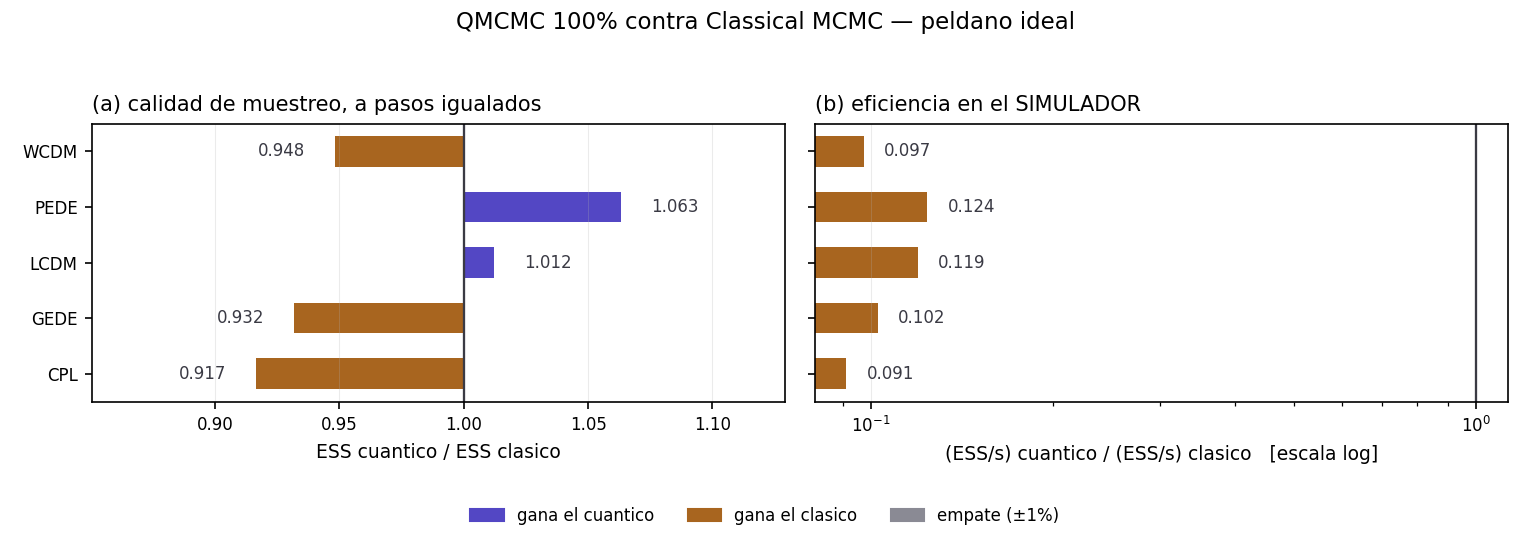
\includegraphics[width=\textwidth]{figs/m_eficiencia.png}
\caption{Dos de cinco modelos quedan a favor del cuántico (PEDE $1.063$,
LCDM $1.012$) y tres en contra (CPL $0.917$, GEDE $0.932$, WCDM $0.948$). La
conclusión honesta es \textbf{empate}.}
\end{figure}

\noindent
\textbf{El panel (a) es la comparación honesta}; es independiente del
hardware. El panel (b) mide el costo de Aer, no el del cómputo cuántico, y
\textbf{no sostiene ninguna afirmación sobre velocidad real}. Está en la
figura porque omitirlo sería peor, no porque se pueda citar como resultado.

\medskip\noindent
Y hay una explicación limpia para el empate, que conviene tener lista: la
propuesta cuántica \emph{no sabe dónde está la posterior} ---los ángulos son
aleatorios, el circuito nunca vio los datos---, así que no tiene mecanismo
por el cual pudiera llegar más rápido. Una razón de $\approx 0.95$ es
exactamente lo que se espera.

% ---------------------------------------------------------------------
\subsection{\texttt{incertidumbre\_reportada}}
\archivo{incertidumbre\_reportada.\{png,pdf\}}

$\sigma(\text{método}) / \sigma(\text{Classical MCMC})$, un punto por
parámetro, la barra vertical es la mediana sobre parámetros.

\contesta{¿La barra de error que reporta cada método es la correcta?}

\begin{figure}[H]
\centering
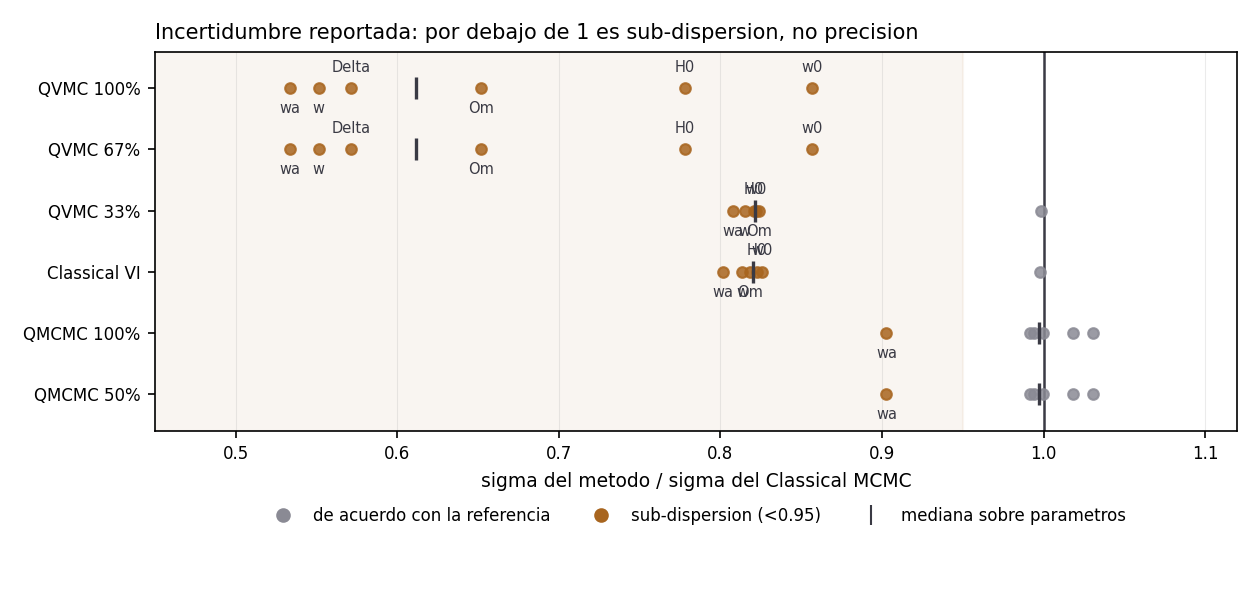
\includegraphics[width=\textwidth]{figs/n_incertidumbre.png}
\caption{Los dos peldaños del QMCMC están sobre el $1$: de acuerdo con la
referencia. Todos los del QVMC están a la izquierda, y bajan al subir la
escalera: $0.82$ con un componente cuántico, $0.65$ con dos o tres.}
\end{figure}

\noindent
\Al{Por debajo de 1 no es precisión: es sesgo.} Si un método reporta
$\pm 0.0035$ donde la verdad es $\pm 0.0269$, un modelo que está a $2\sigma$
aparece a $15\sigma$ y uno anuncia una tensión que no existe.

\medskip\noindent
\textbf{Dos cosas que hay que decir al reportarla.} Primero: la fila
\emph{Classical VI} ya está en $0.80$, y ahí \textbf{no hay nada cuántico} ---
es la asimetría de $\mathrm{KL}(q\|p)$, que castiga poner probabilidad donde
la posterior no tiene y casi no castiga dejar de ponerla donde sí hay, de modo
que el óptimo se mete en el modo y se encoge. Lo que aporta el marco de
ablación es medir que los componentes cuánticos \emph{empeoran} ese sesgo.
Segundo: estos números son \textbf{medianas sobre celdas}, y celda por celda
la razón va de $0.34$ a $1.34$. Reporta la mediana \emph{y} la dispersión;
un árbitro que mire celda por celda va a ver ese $1.34$.

% ---------------------------------------------------------------------
\subsection{\texttt{genetico\_chi2grid}}
\archivo{genetico\_chi2grid.\{png,pdf\}}

$\Delta\chi^2$ del mejor punto de rejilla contra el CGA, un panel por modelo,
eje $x$ = \texttt{n\_bits}, escala simétrica logarítmica. Negativo significa
que el cuántico encontró mejor punto. La punteada marca
$\Delta\chi^2 = 1$.

\contesta{¿El genético cuántico encuentra un punto mejor o peor, y cuánto?}

\begin{figure}[H]
\centering
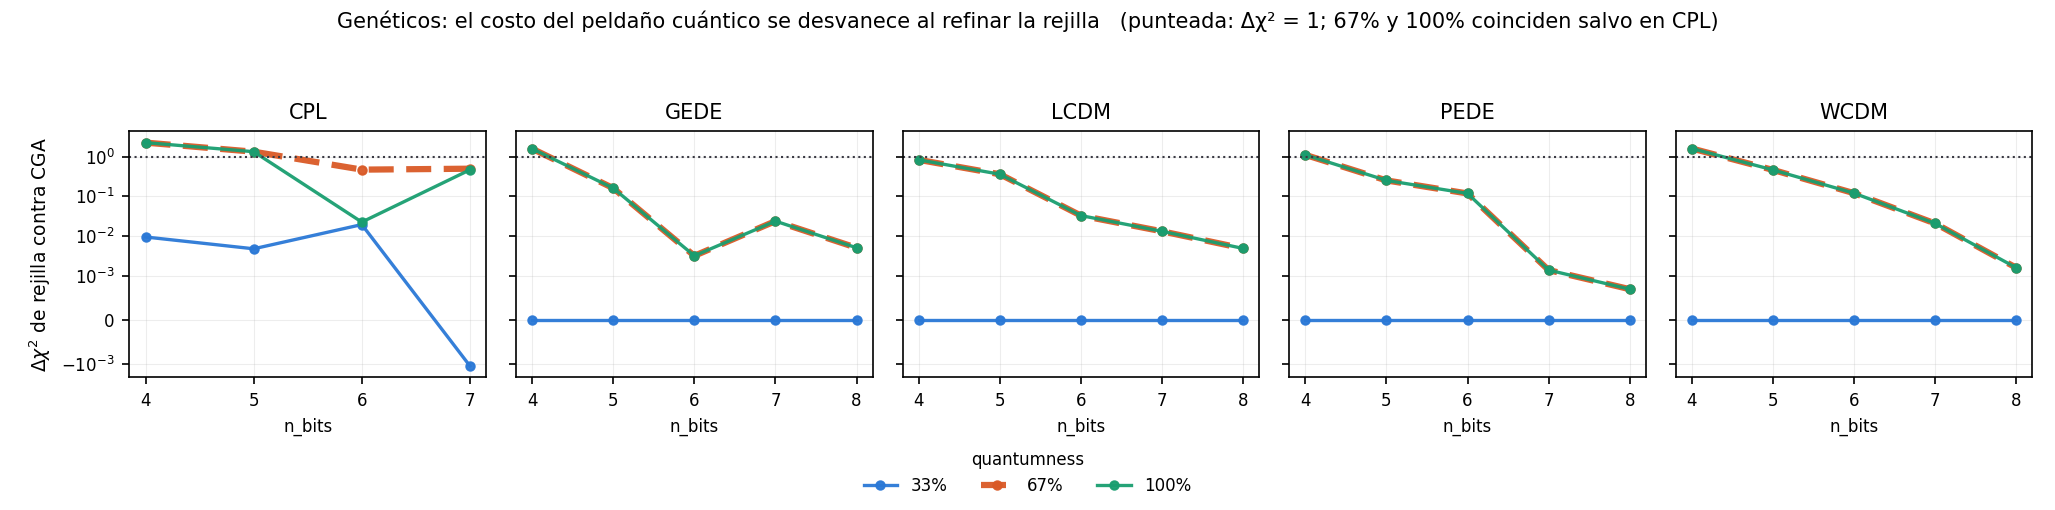
\includegraphics[width=\textwidth]{figs/o_genetico.png}
\caption{El peldaño de $33\%$ (azul) está pegado al cero en los cinco
modelos. Los de $67\%$ y $100\%$ empiezan por encima de $\Delta\chi^2 = 1$ con
$n_b = 4$ y \textbf{caen un orden de magnitud por cada bit que se añade},
hasta $\sim 10^{-3}$ con $n_b = 8$.}
\end{figure}

\noindent
La lectura tiene dos mitades y las dos hay que reportarlas: el signo es
\textbf{consistente en las 24 celdas} ---el cuántico nunca gana, lo cual es un
efecto sistemático real--- pero la \textbf{magnitud se desvanece al refinar la
rejilla}, y sólo 5 de 24 celdas pasan el umbral de relevancia. Decir sólo lo
primero exagera; decir sólo lo segundo esconde un sesgo real.

% ---------------------------------------------------------------------
\subsection{\texttt{modelos\_aic\_bic}}
\archivo{modelos\_aic\_bic.\{png,pdf\}}

$\Delta$AIC y $\Delta$BIC por modelo cosmológico. Las punteadas están en
$2$, $6$ y $10$, que es la escala de Jeffreys.

\contesta{¿Qué modelo cosmológico prefieren los datos?}

\begin{figure}[H]
\centering
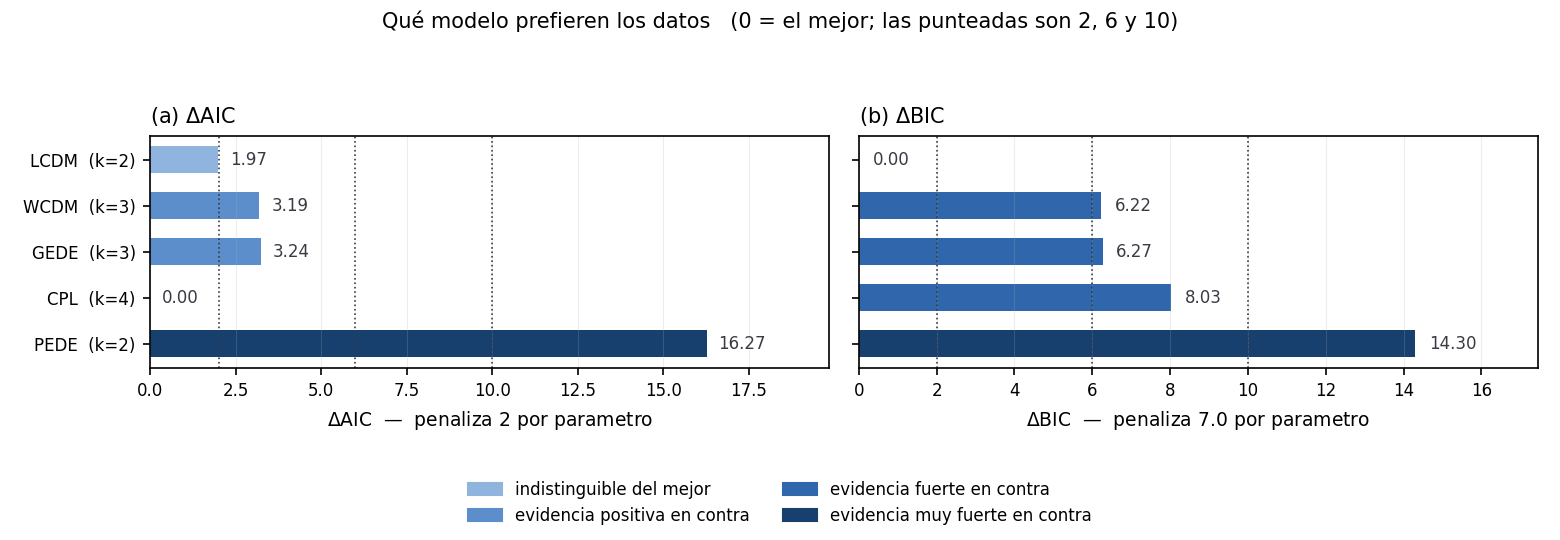
\includegraphics[width=\textwidth]{figs/p_modelos.png}
\caption{Gana CPL por AIC ($\Delta = 0$, con $\Lambda$CDM a $1.97$) y
$\Lambda$CDM por BIC ($\Delta = 0$, con todo lo demás a $6.22$ o más). PEDE
queda rechazado por los dos criterios ($16.27$ y $14.30$).}
\end{figure}

\noindent
\textbf{Que los dos criterios discrepen no es un problema}, y hay que
explicarlo en vez de esconderlo: el BIC cobra $\ln(1099) = 7.0$ unidades de
$\chi^2$ por parámetro extra y el AIC sólo $2$. El parámetro de más de CPL
compra una mejora intermedia --- le alcanza al AIC y no al BIC.

\medskip\noindent
\Al{Cuidado al leerla:} los dos paneles están ordenados por su \emph{propio}
criterio, así que las filas no están en el mismo orden en (a) y en (b).
Comparar a la misma altura entre paneles es un error.

\medskip\noindent
Y un aviso sobre $\chi^2_\nu$: los cinco modelos dan entre $0.967$ y $0.984$.
Todos ajustan de forma aceptable, y por eso \textbf{$\chi^2_\nu$ no sirve
para elegir entre ellos}. Para eso están el AIC y el BIC.

% =====================================================================
\clearpage
\section{Índice rápido}
% =====================================================================

\small
\begin{longtable}{@{}>{\raggedright\arraybackslash}p{5.1cm}>{\raggedright\arraybackslash}p{4.3cm}>{\raggedright\arraybackslash}p{6.2cm}@{}}
\toprule
\textbf{archivo} & \textbf{dónde vive} & \textbf{qué contesta} \\
\midrule
\endhead
\texttt{convergence\_<m>} & \texttt{hpc\_*/}
  & ¿bastan los qubits que usé? \\
\texttt{cost\_<m>} & \texttt{hpc\_*/}
  & qué cuesta en el simulador \\
\texttt{convergence\_<m>\_genetico} & \texttt{hpc\_*/}
  & ¿cuántos bits por gen hacen falta? \\
\texttt{cost\_<m>\_genetico} & \texttt{hpc\_*/}
  & dónde se vuelve impagable el QGA \\
\addlinespace
\texttt{ladder\_trends\_<m>} & \texttt{samplers\_*/model\_*/}
  & qué cambia al encender lo cuántico \\
\texttt{ladder\_summary\_<m>} & \texttt{samplers\_*/model\_*/}
  & los números exactos, en tabla \\
\texttt{ladder\_rhat\_qmcmc\_<m>} & \texttt{samplers\_*/model\_*/}
  & ¿convergió la cadena? \\
\texttt{ladder\_kl\_qvmc\_<m>} & \texttt{samplers\_*/model\_*/}
  & el techo de expresividad del ansatz \\
\texttt{corner\_ladder\_<f>\_<m>} & \texttt{samplers\_*/model\_*/}
  & la fidelidad, vista a ojo \\
\texttt{corner\_ladder\_1to1\_*} & \texttt{samplers\_*/model\_*/}
  & la discrepancia de un peldaño \\
\addlinespace
\texttt{fitness\_<m>\_fitness} & \texttt{genetic\_*/model\_*/}
  & ¿se estancó el genético? \\
\texttt{genetic\_convergence\_<m>} & \texttt{genetic\_*/model\_*/}
  & cómo se encoge la población \\
\addlinespace
\texttt{ruido\_vs\_rejilla\_*} & \texttt{figuras\_*/ruido\_*/}
  & ¿el ruido empeora con el registro? \\
\texttt{ruido\_fijo\_*} & \texttt{figuras\_*/ruido\_*/}
  & qué cuesta el ruido en esta celda \\
\addlinespace
\texttt{eficiencia\_QMCMC*} & \texttt{figuras\_*/comparacion\_*/}
  & ¿más muestras independientes por paso? \\
\texttt{incertidumbre\_reportada} & \texttt{figuras\_*/comparacion\_*/}
  & ¿la barra de error es la correcta? \\
\texttt{genetico\_chi2grid} & \texttt{figuras\_*/comparacion\_*/}
  & ¿el QGA encuentra mejor punto? \\
\texttt{modelos\_aic\_bic} & \texttt{figuras\_*/comparacion\_*/}
  & qué modelo prefieren los datos \\
\bottomrule
\end{longtable}
\normalsize

% =====================================================================
\section{Cómo rehacerlas todas}
% =====================================================================

Ningún paso recalcula nada científico; todos leen los CSV y los logs que la
campaña ya escribió.

\begin{center}
\small
\begin{tabular}{@{}>{\raggedright\arraybackslash}p{6.0cm}>{\raggedright\arraybackslash}p{9.4cm}@{}}
\toprule
\textbf{qué rehace} & \textbf{comando} \\
\midrule
\texttt{convergence\_*}, \texttt{cost\_*}
  & \texttt{python cosmo\_hpc\_runner.py -{}-plot-only CAMPANA} \\
\texttt{ladder\_*}
  & \texttt{python cosmo\_modular\_quantum.py -{}-replot-ladder}\newline
    \texttt{\ \ CAMPANA/samplers\_*/model\_*/resultados\_config.csv} \\
el eje de ruido
  & \texttt{python graficas\_ruido.py CAMPANA -{}-salida SALIDA} \\
las comparaciones
  & \texttt{python comparar\_algoritmos.py CAMPANA -{}-salida SALIDA} \\
todo lo anterior
  & \texttt{bash rehacer\_todo.sh CAMPANA} \\
\bottomrule
\end{tabular}
\end{center}

\noindent
\textbf{Dos avisos sobre rehacer:}

\begin{enumerate}[leftmargin=1.6em]
  \item Los \texttt{ladder\_rhat} y \texttt{ladder\_kl} \textbf{necesitan el
    log de la tarea}, no sólo el CSV: el $\hat{R}$ por paso y el KL por
    iteración no son columnas. Si el log no está a mano, esas dos figuras se
    omiten \emph{en silencio} y el título de las otras sale con
    \texttt{steps=?~|~iters=?}. Ese signo de interrogación es la señal de que
    faltan figuras.
  \item Los \texttt{corner} no se pueden rehacer nunca: necesitan las cadenas.
\end{enumerate}

% =====================================================================
\section{Lo que no hay que hacer con estas figuras}
% =====================================================================

\begin{enumerate}[leftmargin=1.6em]
  \item \textbf{No leer el ESS como métrica de calidad en el variacional.}
    Ahí vale $12288$ en todos los peldaños porque es el número de disparos,
    no una medida de nada.
  \item \textbf{No comparar las \texttt{*\_std} del genético con las $\sigma$
    de los muestreadores.} El genético converge a un punto; su desviación
    mide encogimiento de población, no incertidumbre del parámetro. Por eso
    el script de comparación las imprime en otra sección y con un aviso.
  \item \textbf{No citar una celda cuyo $\hat{R}$ no bajó del umbral.}
  \item \textbf{No comparar \texttt{none} contra un peldaño ruidoso} sin
    mirar antes \texttt{none-counts}.
  \item \textbf{No usar la razón ESS/s como afirmación sobre hardware.} Mide
    Aer.
  \item \textbf{No reportar una diferencia pequeña sin el estudio de
    semillas.} Hoy ninguna celda tiene dos semillas, así que la razón de ESS
    de $0.948$ y los $\Delta\chi^2$ del genético por debajo de $1$
    \textbf{todavía no son defendibles}. Es el hueco más grande que queda.
\end{enumerate}

\end{document}
